\documentclass{article}
\usepackage[utf8]{inputenc}
\usepackage{amsmath}
\usepackage{amssymb}
\usepackage[italian]{babel}
\usepackage{anyfontsize}
\usepackage{hyperref}
\usepackage{nicefrac}
\usepackage{tikz}
\usepackage{pgfplots}
\usepackage{caption}
\usepackage{graphicx}
\usepackage{subcaption}
\usetikzlibrary{patterns,plotmarks}
\usepackage{multirow}

\newcommand{\Zn}{$\mathbb{Z}^n_k$} %comodità, per non riscrivere ogni volta 
\newcommand{\Zii}{$\mathbb{Z}^2_k$}

\begin{document}

\title{\Huge Simulazione di Dinamica di Opinione su Automa Cellulare 
		\[\]\Large Relazione scritta per il corso di \\ Introduzione alla fisica dei sistemi complessi \medskip
		}
\author{Matteo Santini, Matteo Costa}
\date{DATA sticassi}

\maketitle
\tableofcontents
\bigskip

 \section{Abstract}
Il presente progetto si occupa di analizzare il comportamento di una popolazione in un problema di \textit{opinion dynamics} tramite la modellizzazione e la realizzazione simulativa di un automa cellulare. A questo scopo è stato conveniente utilizzare il modello di Ising 2D, opportunamente adattato, per gestire l'evoluzione temporale delle opinioni di individui all'interno di una comunità chiusa. In particolare, è stata studiata la risposta del sistema a tre diverse condizioni ambientali. Si è ritrovato che in generale, per una comunità di questo tipo, la distribuzione delle opinioni tende a rilassare verso due condizioni stazionarie in modalità e tempistiche differenti a seconda del caso in esame.

\section{Introduzione}
\label{Sec:2}
Questo progetto di carattere simulativo è finalizzato allo studio statistico dell'evoluzione temporale di una popolazione di individui dotati di una opinione personale. 
\\ A questo scopo, si decidono di introdurre alcune importanti approssimazioni, cercando di mantenersi sempre il più possibile realistici. Ad esempio, si riduce il parametro di opinione ad una mera variabile discreta a due soli valori possibili ($\pm$1), introducendo così una sorta di analogia al Modello di Ising 2D, che in meccanica statistica permette la descrizione di interazioni locali tra spin nel reticolo cristallino di un materiale condensato per spiegarne l'insorgenza di proprietà magnetiche tramite transizioni di fase interne.
\\ Questo tipo di modello, infatti, si addice alla descrizione di numerosi sistemi fisici complessi, dove è possibile osservare fenomeni di auto-organizzazione, e quello trattato qui di seguito ne è un chiaro esempio. 
\\ Tuttavia, è però necessario avere l'accortezza di adattare le regole di evoluzione canoniche, in quanto a differenza degli atomi nei reticoli cristallini, su cui si è soliti applicare il Modello di Ising, gli individui sono in grado di compiere movimenti in modo simultaneo ad ogni step temporale. Dunque, per introdurre interazioni locali tra gli individui della popolazione si sceglie di definire un parametro di distanza d'influenza, che permetta di selezionare il numero finito di altri individui da cui ciascuno viene influenzato in termini di opinione.
\\ Successivamente, è stata studiata la reazione del sistema in esame a due particolari codizioni, che a seguire andranno sotto il nome di visione parziale e flocking gravitazionale.
\\ La prima consiste sostanzialmente nell'ipotesi di limitare il numero di individui da cui ciascuno viene influenzato ad un valore costante nel tempo ed uniforme sull'intera popolazione. Ciò, infatti, risulta essere un'interessante tema da approfondire, notando che mediamente nella società le singole persone manifestano, più o meno consapevolmente, una propensione ad interagire significativamente con solo poche delle proprie conoscenze effettive.
\[\]
\\ La seconda e ultima, invece, introduce nella dinamica del sistema una sorta di campo gravitazionale che implementi una attratività reciproca tra individui di medesima opinione, simulando così il fenomeno di formazione di comunità omogenee nella società.


\section{Modello Matematico}
\label{Sec:3}

\subsection{Automa Cellulare}
\label{Sec:3.1}
Il seguente modello ad automa cellulare intende porre le basi teoriche matematiche necessarie all'implementazione di una simulazione del comportamento di una popolazione all’interno di uno spazio bidimensionale discretizzato, dato da tutte le coppie di numeri interi nel prodotto cartesiano (0,31]x(0,31] (forse è più corretto [1,L+1]x[1,L+1] con L=31).

\begin{figure}[h]
\centering
\begin{tikzpicture}[
  scale=0.95,
  mydot/.style={
    circle,
    fill=white,
    draw,
    outer sep=0pt,
    inner sep=1pt
  }
]
\draw[step=0.2cm,gray!50!white,very thin] (0,0) grid (6.2,6.2);
\draw[thick,->] (0,0) -- (7,0) node[anchor=north west] {x};
\draw[thick,->] (0,0) -- (0,7) node[anchor=south east] {y};
\foreach \x in {0,5,10,15,20,25,30}
   \draw (\x*0.2 cm,2pt) -- (\x*0.2 cm,-2pt) node[anchor=north] {$\x$};
\foreach \y in {0,5,10,15,20,25,30}
    \draw (2pt,\y*0.2 cm) -- (-2pt,\y*0.2 cm) node[anchor=east] {$\y$};
\filldraw[fill=red!40!red, draw=black] (4,2) circle (0.1cm);
\end{tikzpicture}
\caption{\textit{Rappresentazione grafica dello spazio bidimensionale discretizzato, su cui è disposto arbitrariamente un individuo evidenziato in rosso.}}
\label{fig:1}
\end{figure}

Come è possibile osservare in Figura~\ref{fig:1}, tali coppie compongono le coordinate di tutti i possibili siti dell'automa cellulare, che possono o meno essere occupati dagli individui.
\\ La popolazione in esame è costituita da un numero costante \textit{N=100} di individui, anche detti agenti, i quali sono caratterizzati fondamentalmente da un parametro di opinione personale, che ne definisce univocamente lo stato.
In particolare, questo può assumere solo i valori interi $\pm$1, i quali sono interpretati come l'assenso o il dissenso verso un certo tema politico-sociale.
\bigskip \bigskip
\\ Inoltre, come anticipato in Sezione~\ref{Sec:2}, ad ogni istante dell’evoluzione temporale del sistema, gli agenti sono in grado di compiere in modo simultaneo movimenti all'interno del proprio intorno di Von Neumann di raggio unitario, come rappresentato in Figura~\ref{fig:2}.

\begin{figure}[h]
\centering
\begin{tikzpicture}[
  scale=0.9,
  mydot/.style={
    circle,
    fill=white,
    draw,
    outer sep=0pt,
    inner sep=1pt
  }
]
\draw[step=1cm,gray!50!white,very thin] (0.5,0.5) grid (4.5,4.5);
\fill[fill=green!30!white] (2,2) rectangle (3,3);
\filldraw[fill=green!30!white, draw=black] (2,1) rectangle (3,2);
\filldraw[fill=green!30!white, draw=black] (1,2) rectangle (2,3);
\filldraw[fill=green!30!white, draw=black] (2,3) rectangle (3,4);
\filldraw[fill=green!30!white, draw=black] (3,2) rectangle (4,3);
\filldraw[fill=red!40!red, draw=black] (2.5,2.5) circle (0.5cm);
\put(60,85){$N$};
\put(60,35){$S$};
\put(35,60){$O$};
\put(85,60){$E$};
\end{tikzpicture}
\caption{\textit{Visualizzazione di tutti i siti (in verde) appartenenti all'intorno di Von Neumann di un individuo (in rosso) con relative direzioni (Nord, Sud, Est, Ovest).}}
\label{fig:2}
\end{figure}

Da notare come in realtà sia contemplata anche la possibilità di rimanere fermi, ma limitatamente al caso in cui l'individuo si trovasse occupate tutte le celle nel proprio intorno. Ciò si è reso necessario affinchè in generale sia prediletta la scelta di compiere un movimento rispetto a quella di bloccarsi.
\\ L'effettiva direzione degli spostamenti è scelta stocasticamente tra le quattro permesse (Nord, Sud, Est, Ovest + Stessa posizione nel caso particolare precedentemente descritto), attribuendo a ciascuna di esse una medesima probabilità $\nicefrac{1}{n}$ con n pari al numero di siti liberi adiacenti, tranne quando questo si annulla, in cui invece si permette all’individuo di mantenere la propria posizione, garantendo così sempre la normalizzazione ad 1.
\\ Tali spostamenti all’interno dello spazio discretizzato bidimensionale (0,31]x(0,31] sono vincolati a condizioni al contorno periodiche. Ne segue dunque che topologicamente l’insieme dei siti dell’automa cellulare costituisce una struttura toroidale, esplicitata in Figura~\ref{fig:3} e d'ora in poi indicata con \Zn, dove n=2 e k=31 sono rispettivamente le dimensioni spaziali ed il numero di siti per lato dell'automa cellulare.
\\ Questa scelta implementativa è espressamente motivata dall’obiettivo di evitare moti attrattivi degli individui verso ai bordi, che andrebbero così ad influenzare non trascurabilmente l’evoluzione del sistema.
\\ La dinamica del sistema, di fatto, prevede la scelta del valore di un parametro di controllo, ossia $\delta$ definito come il raggio di influenza, e limitato agli elementi del seguente insieme \{0,...,$\nicefrac{(31-1)}{2}=15$\}. In base al suo valore si decide che l'individuo arbitrario \textit{i} $\in$ $\{1,...,\textit{N} \}$ può interagire solo con coloro la cui posizione è compresa nel suo intorno di influenza $\Delta_{i}(t)$ = $\{ x \in \ $\Zii$ \ | \  \ d(x_{i}(t),x)\leqslant \delta \}$ con \textit{$x_{i}$(t)} come posizione dell'individuo \textit{i} all'istante \textit{t}, mentre \textit{d(x,y)} come metrica di Chebyshev nello spazio discrezzato bidimensionale dell'automa cellulare. 

\begin{figure}[h]
\centering
\begin{tikzpicture}
\begin{axis} 
[view={20}{55}, title={Toroide}, ytick=\empty, xtick=\empty, ztick=\empty, axis line style={draw=none}]
\addplot3
[domain=0:360, y domain=0:360, variable=\u, variable y=\v, mesh, samples=10, z buffer=sort, surf, colormap/blackwhite]
({(3+cos(u))*cos(v)}, {(3+cos(u))*sin(v)}, {sin(u)});
\filldraw[fill=red!40!red, draw=black] (420,210) circle (0.05cm);
\filldraw[fill=red!40!red, draw=black] (200,450) circle (0.05cm);
\filldraw[fill=red!40!red, draw=black] (590,690) circle (0.05cm);
\filldraw[fill=red!40!red, draw=black] (300,550) circle (0.05cm);
\filldraw[fill=blue!40!blue, draw=black] (620,800) circle (0.05cm);
\filldraw[fill=blue!40!blue, draw=black] (455,250) circle (0.05cm);
\filldraw[fill=blue!40!blue, draw=black] (400,900) circle (0.05cm);
\filldraw[fill=red!40!red, draw=black] (380,800) circle (0.05cm);
\filldraw[fill=blue!40!blue, draw=black] (150,680) circle (0.05cm);
\filldraw[fill=blue!40!blue, draw=black] (0,700) circle (0.05cm);
\filldraw[fill=blue!40!blue, draw=black] (400,700) circle (0.05cm);
\filldraw[fill=red!40!red, draw=black] (100,1000) circle (0.05cm);
\end{axis}
\end{tikzpicture}
\caption{Caption}
\label{fig:3}
\end{figure}

\bigskip \bigskip
Da notare come la validità delle condizioni al contorno periodiche comporta la costruzione di range d'influenza, anche detti intorni di Moore estesi, molto particolari, di cui sono riportati alcuni esempi in Figura~\ref{fig:3}.

\begin{figure}[h]
\centering
\begin{tikzpicture}[
  scale=0.7,
  mydot/.style={
    circle,
    fill=white,
    draw,
    outer sep=0pt,
    inner sep=1pt
  }
]
\fill[fill=green!30!white] (1,2.5) rectangle (3.5,5);
\fill[fill=green!30!white] (7,0) rectangle (8.5,2);
\fill[fill=green!30!white] (7,5.5) rectangle (8.5,6);
\fill[fill=green!30!white] (12,0) rectangle (13,2);
\fill[fill=green!30!white] (12,5.5) rectangle (13,6);
\draw[step=0.5cm,gray!50!white,very thin] (-1,0) grid (5,6);
\draw[step=0.5cm,gray!50!white,very thin] (6.99,0) grid (13,6);
\filldraw[fill=red!40!red, draw=black] (2.25,3.75) circle (0.25cm);
\filldraw[fill=red!40!red, draw=black] (7.25,0.75) circle (0.25cm);
\end{tikzpicture}
\caption{\textit{Intorni di Moore estesi di raggio 2 in due differenti casi.}}
\label{fig:4}
\end{figure}

In questi termini, una volta noto lo stato del sistema dato dalla conoscenza della corrispondenza $S(t): i \rightarrow s(i,t), $ è possibile quantificare l'influenza a cui un individuo generico $\textit{i} \in \{1,...,\textit{N} \}$ è soggetto all'istante temporale $\textit{t}$ come il seguente parametro reale nell'intervallo compatto $[-1,+1]$

\begin{equation}
    \sigma(i,t) = \sum_{ \{ j \ | \ x_{j} \in \Delta_{i} \} } s(j, t)p(M_{i}(t))
    \medskip
    \label{Eq:1}
\end{equation}

che appunto consiste di una media uniformemente pesata degli stati, ossia delle opinioni, \textit{s(j,t)} degli individui \textit{j} la cui posizione è compresa nell'intorno d'influenza $\Delta_{i}(t)$ precedentemente definito all'istante \textit{t}. Infatti, i coefficienti moltiplicativi \textit{p}($M_{i}(t)$) = $\nicefrac{1}{M_{i}(t)}$, con $M_{i}(t)$ pari al numero di agenti influenti su \textit{i} all'istante \textit{t}, non dipendono dall'indice \textit{j} su cui viene eseguita l'operazione di sommatoria e soddisfano la condizione di normalizzazione:

\begin{equation}
    \sum_{ \{ j \ | \ x_{j} \in \Delta_{i} \} } p(M_{i}(t)) = M_{i}(t) \cdot p(M_{i}(t)) =    M_{i}(t) \cdot \left ( \frac{1}{M_{i}(t)} \right ) = 1.
    \medskip
    \label{Eq:2}
\end{equation}

Per finire, si implementa l'evoluzione temporale locale dell'opinione dell'agente \textit{i} valutando l'influenza associata $\sigma(i,t)$  calcolata in Equazione~\ref{Eq:1} tramite la funzione a valori interi $I_{A}$ che ne caratterizza l'andamento ed è così definita

\begin{equation}
    s(i,t+1) = I_A(\sigma(i,t)) = sign(\sigma(i,t)).
    \medskip
    \label{Eq:3}
\end{equation}

La scelta di tale regola di evoluzione del sistema determina una forte sensibilità degli individui all'influenza percepita, perchè non appena questa assume un segno discorde dalla loro opinione si verifica una transizione di stato \mbox{(+1 $\longleftrightarrow$ -1)} nonostante il suo modulo risulti essere $|\sigma(i,t)| \ll 1$.
\\ Al fine, quindi, di rallentare la dinamica delle opinioni, è stato introdotto un ulteriore parametro \textit{T}, definito positivo e analogo alla temperatura nei sistemi fisici, che moduli la velocità di rilassamento alla distribuzione stazionaria in termini di probabilità di transizione di stato $ \pi_{\pm}(T) = \pi(T) = \tanh (T)$.
\\ Per considerazioni di convenienza computazionale, è stato scelto un valore costante $T=1$.

\bigskip
\begin{figure}[h]
\centering
\begin{tikzpicture}[line cap=round, line join=round,
                            x=3.0cm, y=2.0cm, scale=1]
\draw [->,color=black, line width=1.0pt] (-0.05,0) -- (2.5,0);
\foreach \x in {1}
\draw [shift={(\x,0)}, color=black] (0pt,2pt)
-- (0pt,-2pt) node [below] {$\x$};
\draw [color=black] (2.5,0) node [anchor= north west] {$T$};
\draw [->,color=black, line width=1.0pt] (0,-0.1) -- (0,2);
\foreach \y in {0.7616,1}
\draw [shift={(0,\y)}, color=black] (2pt,0pt)
-- (-2pt,0pt) node[left] {$\y$};
\draw [color=black] (0,2) node [anchor= south east] {$\pi (T)$};
\draw [color=black] (0pt,-10pt) node [left] {$0$};
\draw [domain=0:2.4, line width=1.0pt, color=blue] plot (\x,{tanh(\x)});
\draw [dashed, color=gray, line width=0.6pt] (1,0) -- (1,1);
\draw [dashed, color=gray, line width=0.6pt] (0,1) -- (2.45,1);
\draw [dashed, color=gray, line width=0.6pt] (0,0.7616) -- (1,0.7616);
\filldraw[fill=white, draw=blue, line width=0.8pt] (1,0.7616) circle (0.08cm);
\end{tikzpicture}
\caption{\textit{Andamento caratteristico della probabilità di transizione di stato al variare della temperatura T, con il valore scelto per le simulazioni in evidenza.}}
\label{fig:5}
\end{figure}

\bigskip \bigskip
\subsection{Visione Parziale}
\label{Sec:3.2}

Come anticipato in Sezione \ref{Sec:2}, il sistema appena descritto viene sottoposto ad una condizione esterna globale, detta visione parziale. Questa prevede l'introduzione di un ulteriore parametro di controllo discreto $\eta$ e la scelta di un valore fissato arbitrario di distanza d'influenza (ad esempio, nelle simulazioni $\delta=4$).
\\ Il parametro $\eta$ decide il numero massimo di individui da cui ciascuno può essere influenzato, ed è costante nel tempo, uniforme su tutta la popolazione e limitato agli elementi del seguente insieme $\{ 1, ..., (2\delta+1)(2\delta+1)-1=80\}$, come si può dedurre da Figura \ref{fig:6}.

\begin{figure}[h]
\centering
\begin{tikzpicture}[
  scale=0.95,
  mydot/.style={
    circle,
    fill=white,
    draw,
    outer sep=0pt,
    inner sep=1pt
  }
]
\fill[fill=green!30!white] (1,1) rectangle (2.8,2.8);
\draw[step=0.2cm,gray!50!white,very thin] (0,0) grid (4,4);
\draw[thick,->] (1,4.1) -- (2.8,4.1) node[] {};
\draw[thick,->] (2.8,4.1) -- (1,4.1) node[] {};
\draw[thick,->] (4.1,1) -- (4.1,2.8) node[] {};
\draw[thick,->] (4.1,2.8) -- (4.1,1) node[] {};
\filldraw[fill=red!40!red, draw=black] (1.9,1.9) circle (0.1cm);
\put(35,118){$(2\delta+1)$};
\put(115,48){$(2\delta+1)$};
\end{tikzpicture}
\caption{\textit{Rappresentazione grafica dell'intorno d'influenza $\Delta$ di un individuo, posizionato arbitrariamente, con $\delta$=4. Utile per comprendere che necessariamente il limite superiore di $\eta$ debba essere il numero di siti in $\Delta$, escluso quello occupato dall'individuo stesso.}}
\label{fig:6}
\end{figure}

Oltre a questa peculiaretà, la dinamica e l'evoluzione temporale delle opinioni seguono sostanzialmente le medesime regole valide per l'automa cellulare, specificate in Sezione \ref{Sec:3.1}.


\subsection{Flocking Gravitazionale}
\label{Sec:3.3}

In questo modello ad automa cellulare sono stati inseriti due campi che agiscono su tutti gli individui della stessa opinione attraverso una forza attrattiva proporzionale a $\nicefrac{1}{r^2}$. Fisicamente questi campi corrispondono ad una coppia di campi gravitazionali

\begin{equation}
\begin{aligned}
\begin{cases}
F_x:  \mathbb{Z}^2_k \rightarrow \mathbb{R}^2 \\
F_y:  \mathbb{Z}^2_k \rightarrow \mathbb{R}^2 
\end{cases}
\end{aligned}
\end{equation}

la cui forza agente tra due individui \textit{i}, \textit{j} a distanza $\vec{r}_{x}$ lungo le ascisse e $\vec{r}_{y}$ lungo le ordinate, aventi la medesima opinione è

\begin{equation}
\begin{aligned}
    \vec{F}_x^{(i,j)} =& \dfrac{Gm_im_j}{r_x^2} \hat{r_x} \quad\quad con \quad i\neq j\\
    \vec{F}_y^{(i,j)} =& \dfrac{Gm_im_j}{r_y^2} \hat{r_y} \quad\quad con \quad i\neq j
\end{aligned}
\end{equation}

nell'ipotesi in cui tutti gli individui abbiano massa m=1 e che la costante gravitazionale sia G=10, per facilitare l'implementazione del modello (vedi Figura \ref{Fig:7}). 

\begin{figure}[h]
\centering
\begin{tikzpicture}[
  scale=0.7,
  mydot/.style={
    circle,
    fill=white,
    draw,
    outer sep=0pt,
    inner sep=1pt
  }
]
\draw[step=0.3cm,gray!50!white,very thin] (-1,0) grid (5,6);
\filldraw[fill=red!40!red, draw=black] (1.95,3.15) circle (0.1cm);
\draw [-latex] (2.05, 3.15) -- (4.05, 3.15);
\draw [-latex] (1.85, 3.15) -- (-0.15, 3.15);
\draw [-latex] (1.95, 3.25) -- (1.95, 5.25);
\draw [-latex] (1.95, 3.05) -- (1.95, 1.15);
\draw (0.65,5.2) node[] {} node[right] {$+F_y$};
\draw (1.95,1.2) node[] {} node[right] {$-F_y$};
\draw (-0.5,2.75) node[] {} node[right] {$-F_x$};
\draw (3.75,3.5) node[] {} node[right] {$+F_x$};
\end{tikzpicture}
\caption{\textit{Rappresentazione grafica delle possibili combinazioni di coppie di forze agenti su un individuo}}.
\label{Fig:7}
\end{figure}

L'introduzione di campi di questo tipo favorisce il fenomeno del \textit{flocking}, ossia la formazione di assembramenti tra individui della stessa opinione. Questo fenomeno introduce degli attrattori nella dinamica degli individui nello spazio \Zii: come si osserva in una comunità reale, persone aventi opinione politica affine tendono a stare assieme mentre, persone immerse in un ambiente in cui la propria ideologia politica non è ben vista, tendono a spostarsi dove ci sono individui che condividono la propria opinione.
\\
Le condizioni al contorno periodiche, che determinano la struttura toroidale dell'automa cellulare come spiegato in Sezione \ref{Sec:3.1}, possono rappresentare un difficoltà aggiuntiva ai fini della dinamica. Infatti, per ognuna delle due forze agenti tra due individui ci sono sempre due possibili distanze, ma è necessario che il modulo, direzione e verso di queste forze siano univocamente definiti per ogni coppia. Ad esempio, se consideriamo solo le forze agenti in direzione x, per ogni coppia di individui \textit{i}, \textit{j}, esiste una distanza che segue il verso positivo dell'asse delle ascisse, indicata con $r_x^+$, e una che va in senso opposto, denominata invece $r_x^-$. Assumendo una considerazione del tutto analoga anche per le forze agenti in y, le distanze utilizzate per i due campi vettoriali $\vec{F}^{(i,j)}_x$ e $\vec{F}^{(i,j)}_y$ sono state calcolate in base alle seguenti definizioni: rispettivamente,

\begin{equation}
\begin{aligned} 
&r_x(i,j) = min\{|r_x^+|, |r_x^-|\}\\
&r_y(i,j) = min\{|r_y^+|, |r_y^-|\}.
\end{aligned}
\end{equation}

Chiaramente, è necessario imporre delle ulteriori condizioni sulle forze per evitare dei punti singolari. Innanzitutto, si assume che se $r_x(i,j)$ o $r_y(i,j)$ si annulla, allora la forza corrispondente in x o y sarà nulla. È anche evidente che non è possibile avere entrambe $r_x(i,j)$ e $r_y(i,j)$ uguali a zero, perchè questo va in contraddizione con la richiesta $i\neq j$ (gli individui non si possono compenetrare). Allora, viene subito da domandarsi quando $\vec{F}^{(i,j)}_x$ e $\vec{F}^{(i,j)}_y$ possano essere entrambe nulle: questo caso particolare richiede delle considerazioni di carattere geometrico che risiedono nella struttura del toroide topologico. Quando, infatti, si realizza la condizione $r_x(i,j) = min\{|r_x^+|, |r_x^-|\} = |r_x^+| = |r_x^-|$ (ovvero quando le due distanze coincidono), si richiede che $\vec{F}^{(i,j)}_x$ = 0. Analogamente, ciò vale anche per $\vec{F}^{(i,j)}_y$, quando $r_y(i,j) = min\{|r_y^+|, |r_y^-|\} = |r_y^+| = |r_y^-|$. Ne è un chiaro esempio la configurazione in Figura \ref{Fig:8}.

\begin{figure}[hb]
\centering
\begin{subfigure}[h]{0.48\textwidth}
\centering
\begin{tikzpicture}[
  scale=0.7,
  mydot/.style={
    circle,
    fill=white,
    draw,
    outer sep=0pt,
    inner sep=1pt
  }
]
\draw[step=0.3cm,gray!50!white,very thin] (-1,0) grid (5,6);
\filldraw[fill=red!40!red, draw=black] (2.25,3.15) circle (0.1cm);
\filldraw[fill=red!40!red, draw=black] (-0.75,3.15) circle (0.1cm);
\end{tikzpicture}
\end{subfigure}
\hfill
\begin{subfigure}[h]{0.48\textwidth}
         \centering
\begin{tikzpicture}
\begin{axis} 
[view={0}{100}, ytick=\empty, xtick=\empty, ztick=\empty, axis line style={draw=none}]
\addplot3
[domain=0:360, y domain=0:360, variable=\u, variable y=\v, mesh, samples=10, z buffer=sort, surf, colormap/blackwhite]
({(3+cos(u))*cos(v)}, {(3+cos(u))*sin(v)}, {sin(u)});
\filldraw[fill=red!40!red, draw=black] (90,320) circle (0.06cm);
\filldraw[fill=red!40!red, draw=black] (710,300) circle (0.06cm);
\end{axis}
\end{tikzpicture}
\end{subfigure}
\caption{\textit{Esempio in cui la forza agente tra i due individui in rosso è nulla. A sinistra la rappresentazione nell'automa cellulare di questa situazione, a destra la sua corrispondenza sul toroide \Zii  che tiene conto delle periodic boundary conditions.}}
\label{Fig:8}
\end{figure}

Una volta determinati i contributi attrattivi $F_x^{(i,j)}(t)$ e $F_y^{(i,j)}(t)$ dovuti a tutti gli accoppiamenti possibili dell'individuo arbitrario \textit{i} con i suoi simili \textit{j} nella popolazione, si può passare alla stima delle forze gravitazionali totali $F_x^{(i)}(t)$ e $F_y^{(i)}(t)$ agenti proprio su \textit{i} all'istante temporale \textit{t} tramite le seguenti somme vettoriali

\begin{equation}
\begin{aligned}
    \vec{F}_x^{(i)}(t) = \sum_{ \{ j \ | \ s(j,t)=s(i,t) \} } \vec{F}_x^{(i,j)}(t) \\
    \vec{F}_y^{(i)}(t) = \sum_{ \{ j \ | \ s(j,t)=s(i,t) \} } \vec{F}_y^{(i,j)}(t).
\end{aligned}
\end{equation}

Sono questi vettori, dunque, i veri responsabili della particolare dinamica di \textit{flocking} gravitazionale.
\\ In base al loro modulo, direzione e verso vengono modificate le probabilità di scelta della direzione di spostamento dei singoli individui all'interno del proprio intorno unitario di Von Neumann, minimizzando progressivamente la distanza tra gli individui di egual opinione, in modo da formare delle regioni ad alta densità di individui e regioni a bassa densità di individui. 
\\ In particolare, la distribuzione di probabilità nella scelta della direzione degli spostamenti di ciascun individuo non sarà più uniforme, come descritto in Sezione \ref{Sec:3.1} per l'automa cellulare "imperturbato", ma polarizzata verso le direzioni parallele e concordi alle forze risultanti in modo tale da rispettare sempre la normalizzazione ad 1.
\\ Ciò è stato realizzato riscalando la crescita o decrescita di probabilità di scelta di una certa direzione rispetto al modulo quadro della forza totale risultante, ossia $|\vec{F}_{TOT}^{(i)}(t)|^2 =|\vec{F}_x^{(i)}(t)|^2+|\vec{F}_y^{(i)}(t)|^2$, nel seguente modo:

\begin{equation}
\begin{aligned}
\begin{cases}
P_x^{(i, \pm)}(t) = \dfrac{1}{4} \left ( 1 \pm \dfrac{|\vec{F}_x^{(i)}(t)|^2}{|\vec{F}_{TOT}^{(i)}(t)|^2} \right ) \\ \\
P_y^{(i, \pm)}(t) = \dfrac{1}{4} \left ( 1 \pm \dfrac{|\vec{F}_y^{(i)}(t)|^2}{|\vec{F}_{TOT}^{(i)}(t)|^2} \right )
\end{cases}
\end{aligned}
\end{equation}

dove i pedici x ed y distinguono la direzione di cui si sta valutando la probabilità, mentre gli apici $\pm$ specificano rispettivamente se il verso è quello concorde o discorde alla relativa forza gravitazionale.
\\ Tuttavia, definizioni di questo tipo possono essere valide soltanto nel caso banale in cui si considerino tutti i siti adiacenti come disponibili, perchè esclusivamente in tale configurazione sarebbe garantita la normalizzazione ad 1.
\\ Di conseguenza, nel caso più realistico di occupazione parziale o completa dei posti adiacenti ad un certo individuo, si inizia con l'imposizione di annullamento della probabilità di spostamento nelle direzioni già impegnate. Dunque, si ridistribuiscono i valori, che nel caso normale sarebbero stati assegnati a tali probabilità, affinchè sia conservata più inalterata possibile la dinamica del sistema e allo stesso tempo sia soddisfatta la normalizzazione ad 1 richiesta.
\\ Infatti, ipotizzando che un individuo \textit{i} arbitrario abbia un numero di siti adiacenti liberi pari a \textit{n=2} e che quelli occupati siano uno in direzione x e verso discorde alla forza $\vec{F}_x^{(i)}$ e l'altro in direzione y e verso concorde alla forza $\vec{F}_x^{(i)}$, le probabilità di scelta saranno date da

\begin{equation}
\begin{aligned}
\begin{cases}
P_x^{(i, +)} = \dfrac{1}{4} \left ( 1 + \dfrac{|\vec{F}_x^{(i)}|^2}{|\vec{F}_{TOT}^{(i)}|^2} \right ) + \dfrac{1}{4n} \left ( 1 - \dfrac{|\vec{F}_x^{(i)}|^2}{|\vec{F}_{TOT}^{(i)}|^2} \right ) + \dfrac{1}{4n} \left ( 1 + \dfrac{|\vec{F}_y^{(i)}|^2}{|\vec{F}_{TOT}^{(i)}|^2} \right ) \\
P_x^{(i, -)} = 0 \\
P_y^{(i, +)} = 0 \\
P_y^{(i, -)} = \dfrac{1}{4} \left ( 1 - \dfrac{|\vec{F}_y^{(i)}|^2}{|\vec{F}_{TOT}^{(i)}|^2} \right ) + \dfrac{1}{4n} \left ( 1 - \dfrac{|\vec{F}_x^{(i)}|^2}{|\vec{F}_{TOT}^{(i)}|^2} \right ) + \dfrac{1}{4n} \left ( 1 + \dfrac{|\vec{F}_y^{(i)}|^2}{|\vec{F}_{TOT}^{(i)}|^2} \right )
\end{cases}
\end{aligned}
\end{equation}

e così soddisfino semplicemente la condizione di normalizzazione ad 1.
\\ Da notare come, similarmente al modello ad automa cellulare descritto in Sezione \ref{Sec:3.1}, per \textit{n=0} è permessa la possibilità di rimanere fermi tra un istante temporale e quello successivo.

%\begin{equation}
%P_x^{(i, +)} + P_x^{(i, -)} + P_y^{(i, +)} + P_y^{(i, -)} = 1 + \dfrac{|\vec{F}_x^{(i)}|^2}{4|\vec{F}_{TOT}^{(i)}|^2} - \dfrac{|\vec{F}_x^{(i)}|^2}{4|\vec{F}_{TOT}^{(i)}|^2} + \dfrac{|\vec{F}_y^{(i)}|^2}{4|\vec{F}_{TOT}^{(i)}|^2} - \dfrac{|\vec{F}_y^{(i)}|^2}{4|\vec{F}_{TOT}^{(i)}|^2} = 1.
%\end{equation}


\section{Analisi e Risultati}
\label{Sec:4}

\subsection{Distanza di Influenza}
\label{Sec:4.1}

L'analisi temporale dell'osservabile di magnetizzazione, definito in analogia al Modello di Ising 2D come

\begin{equation}
M(t) = \dfrac{1}{N} \sum_{i = 0}^{N} s(i,t)
\end{equation}

permette lo studio del comportamento medio del sistema nell'arco delle simulazioni.
\\ In questo modo, applicando valori sempre maggiori del parametro di distanza d'influenza $\delta$, è stato possibile osservare come ciò comporti una significativa accelerazione della dinamica. Infatti, gli esempi in Figura \ref{Fig:9} riportano chiaramente che il tempo necessario al raggiungimento di una delle due distribuzioni stazionarie ("Tutti +1" e "Tutti -1") si riduce sensibilmente all'aumentare di $\delta$.

\begin{figure}[h]
{\centering\par
\makebox[0 pt]{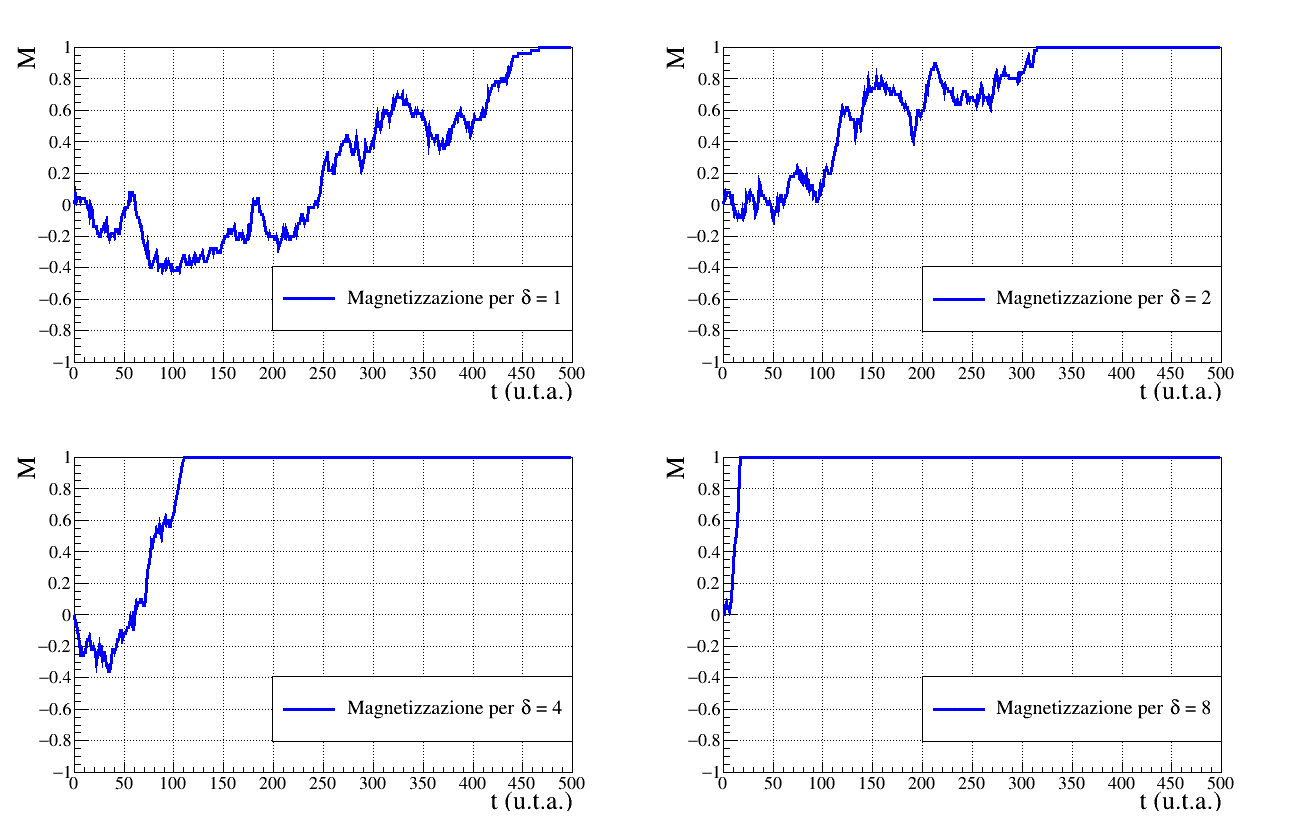
\includegraphics[width=1.3\linewidth]{distance_magnetization_graphs.png}}
\par}
\caption{\textit{Grafici riguardanti l'evoluzione temporale della magnetizzazione per quattro valori di distanza d'influenza (in ordine dall'alto verso il basso e da sinistra a destra: $\delta$ = 1, 2, 4, 8) in simulazioni da 500 steps temporali ciascuna.}}
\label{Fig:9}
\end{figure}

Inoltre, per analizzare più dettagliatamente la proprietà di $\delta$ di ridurre le tempistiche del sistema sono stati raccolti ulteriori dati riguardanti i tempi di decisione $\tau$, ossia gli intervalli di tempo necessari a ciascun individuo di cambiare la propria opinione.
\\ La loro rappresentazione grafica, in Figura  \ref{Fig:10}, ha evidenziato un andamento tipico di una legge a potenza, come ha dimostrato il fit rispetto

\begin{equation}
f(\tau) = c \ \tau ^{a}
\label{Eq:11}
\end{equation}

con \textit{c} e \textit{a} costanti, i cui valori stimati sono in Tabella . 

\begin{center}
\begin{tabular}{ |c|c|c|c| } 
\hline
 Simulazioni & \textit{c} & \textit{a} \\
\hline
\multirow{4}{4em}{$\delta$ = 1 \\$\delta$ = 2 \\$\delta$ = 4 \\$\delta$ = 8 } & 0.0162 $\pm$ 0.0009 & -0.35 $\pm$ 0.01 \\ 
& 0.048 $\pm$ 0.002 & -0.61 $\pm$ 0.01 \\ 
& 0.140 $\pm$ 0.004 & -0.92 $\pm$ 0.03 \\ 
& 0.36 $\pm$ 0.01 &  -1.27 $\pm$ 0.07 \\
\hline
\end{tabular}
\end{center}

\begin{figure}[h]
{\centering\par
\makebox[0 pt]{
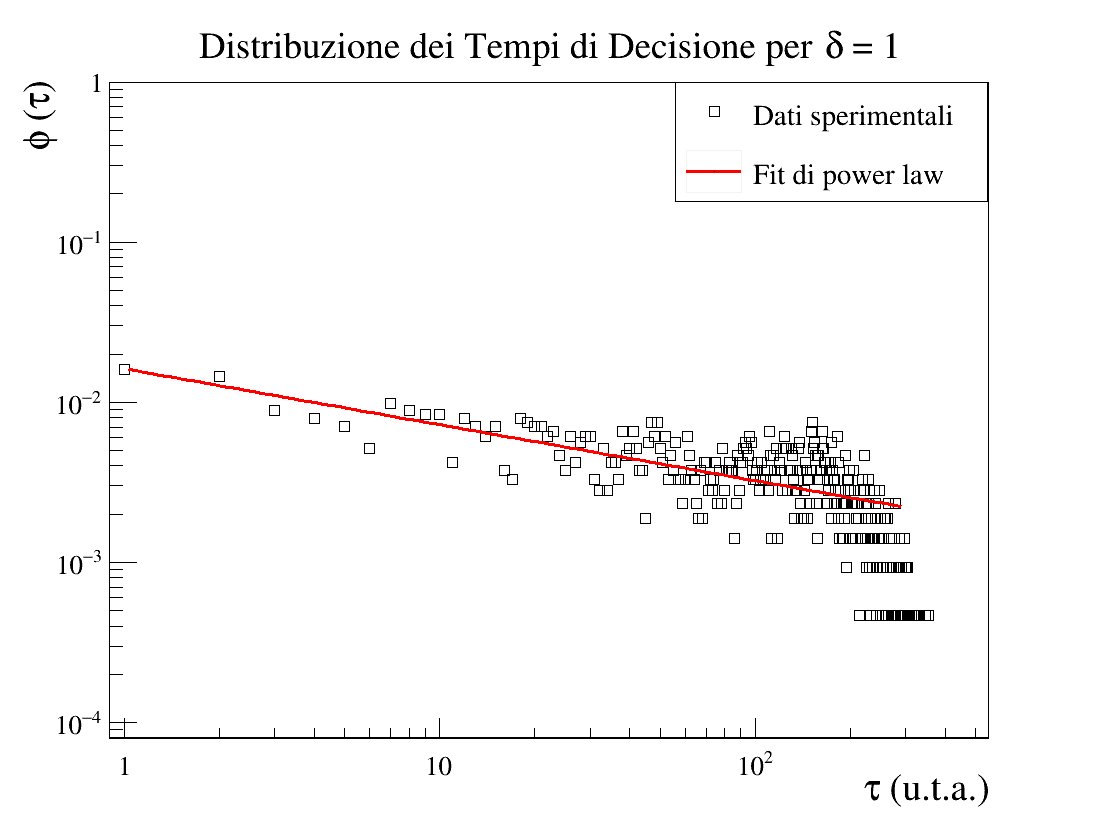
\includegraphics[width=0.57\linewidth]{time_graph_d1.png}
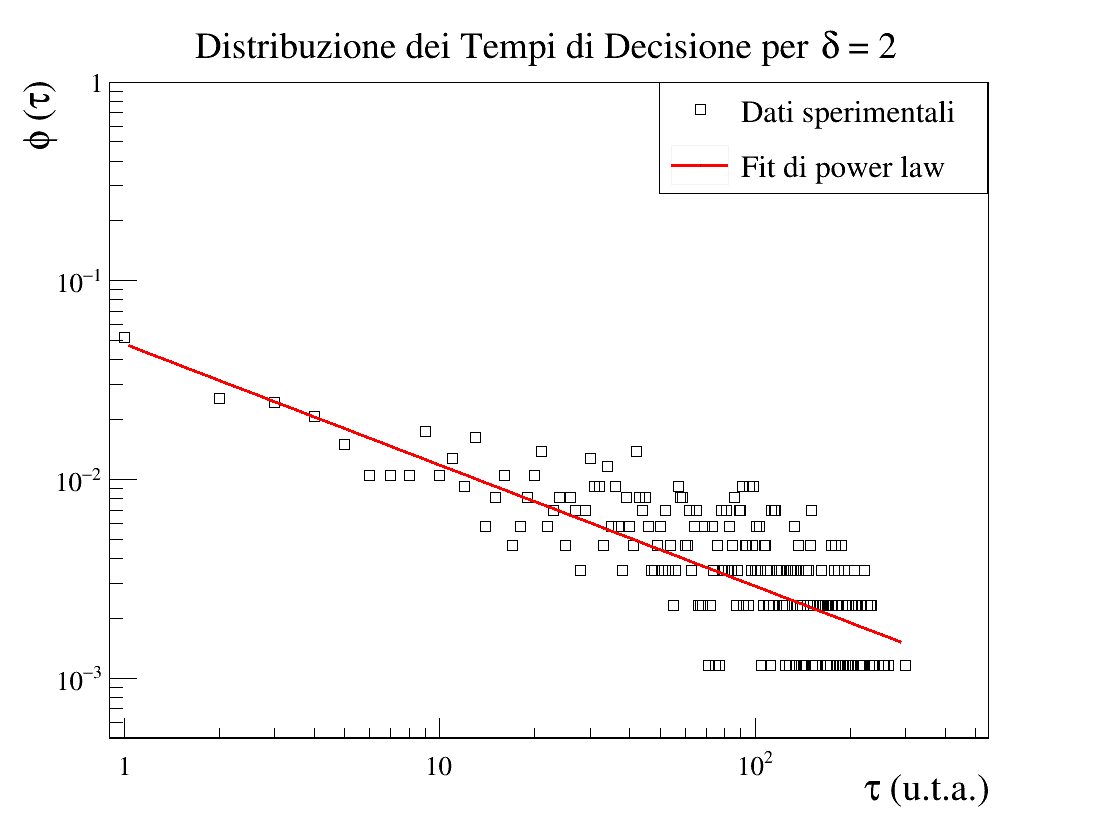
\includegraphics[width=0.57\linewidth]{time_graph_d2.png}}
\par}
{\centering\par
\makebox[0 pt]{
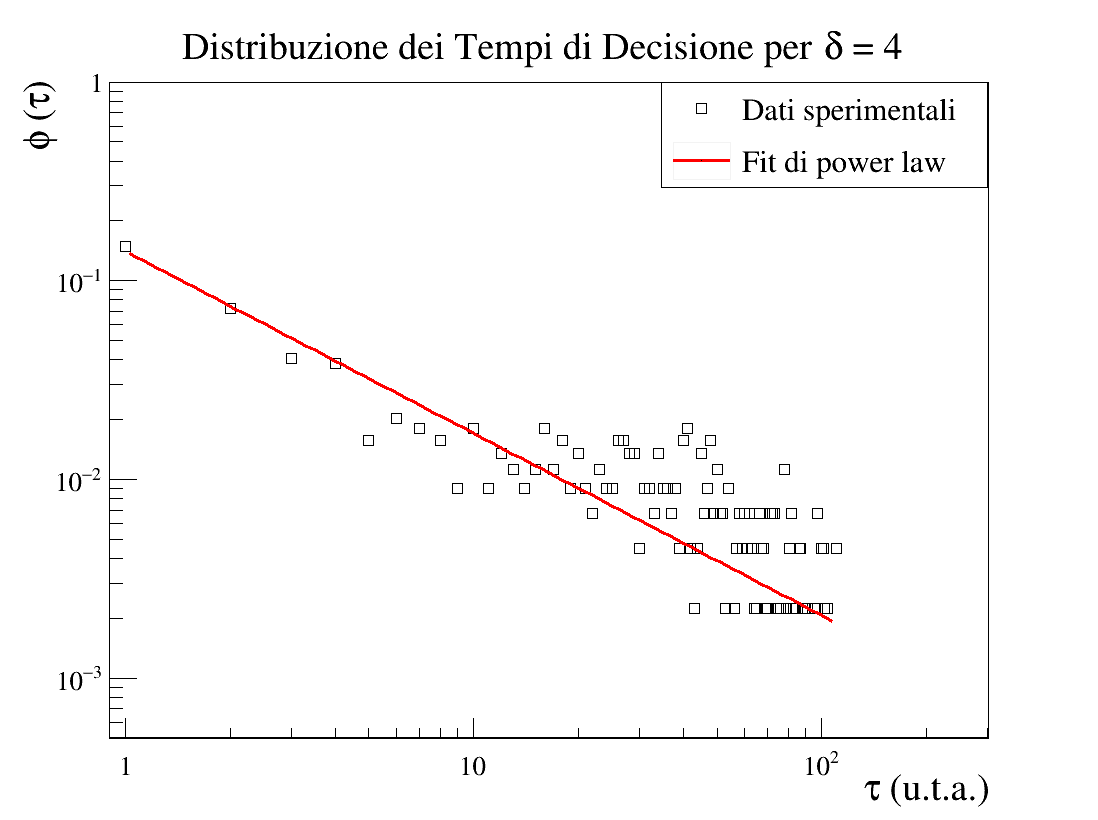
\includegraphics[width=0.57\linewidth]{time_graph_d4.png}
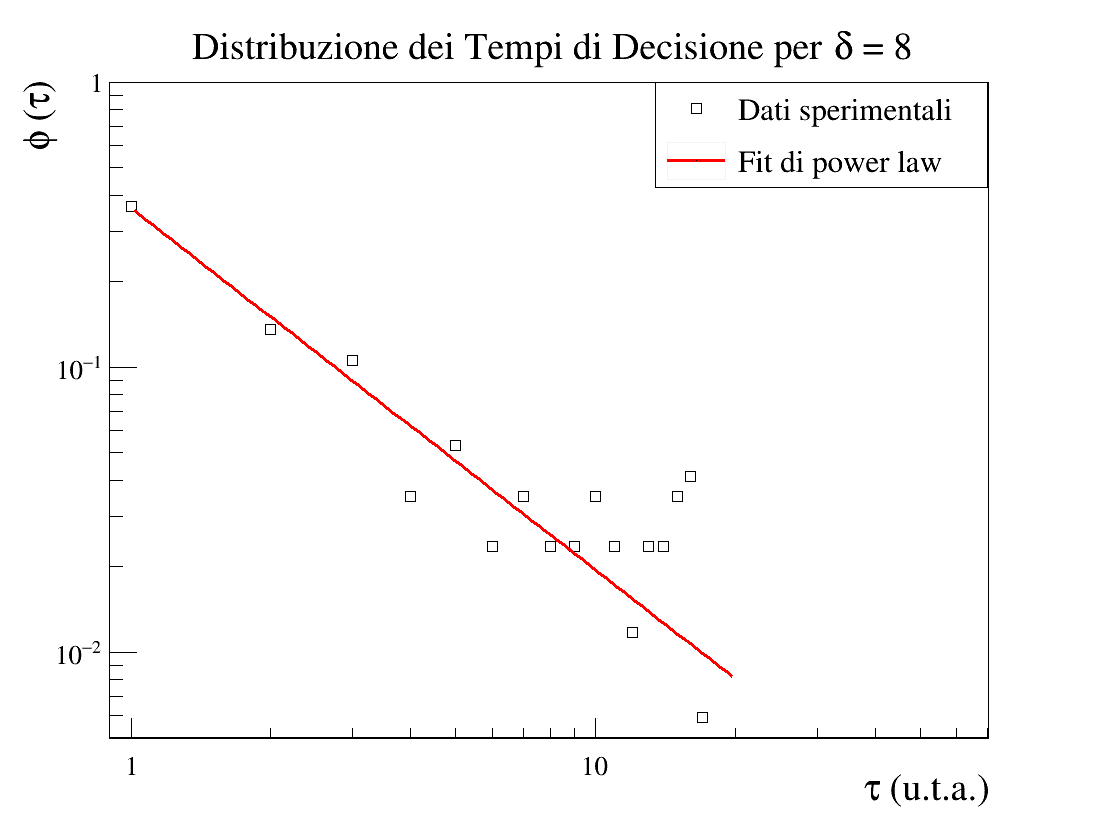
\includegraphics[width=0.57\linewidth]{time_graph_d8.png}}
\par}
\caption{\textit{Illustrazioni delle distribuzioni $\phi(\tau)$ dei tempi di decisione $\tau$, ottenute dalle medesime simulazioni, la cui magnetizzazione è riportata in Figura \ref{Fig:9}, assieme al relativo fit di power law in rosso.  }}
\label{Fig:10}
\end{figure}

\subsection{Influenza delle Condizioni Iniziali}
\label{Sec:4.4}

Uno degli scopi principali di questa tipolologia di modelli di \textit{opinion dynamics} è quello di comprendere le eventuali correlazioni tra condizioni iniziali e distribuzioni stazionarie del sistema.
\\ A tal fine, è stata fatta variare la concentrazione iniziale $c_{-}^{in} = (\nicefrac{N_{-}^{in}}{N})$ di agenti d'opinione -1 nella popolazione in esame e per ciascuno dei valori selezionati sono state svolte 500 simulazioni, così da avere un campione statistico valido per la stima della probabilità di osservazione dei due stati stazionari noti.

\begin{figure}[h]
\centering
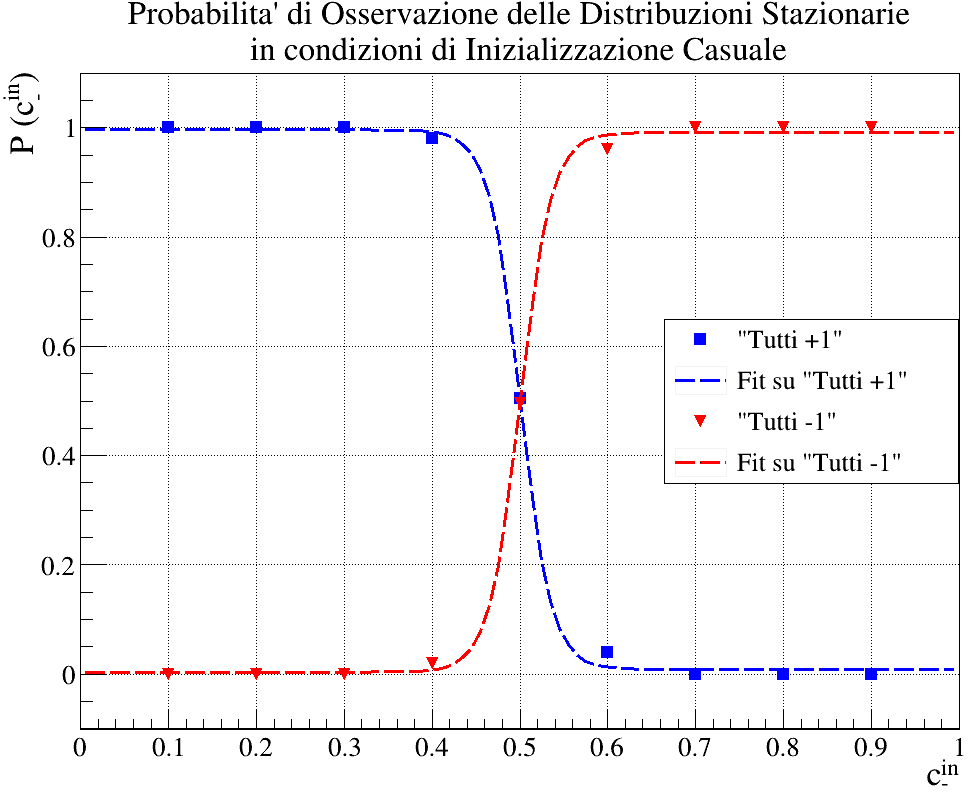
\includegraphics[width = \linewidth]{random_prob_graph.png}
\caption{\textit{bla bla bla}}
\label{Fig:11}
\end{figure}

Come è possibile visualizzare in Figura \ref{Fig:10}, l'andamento di queste probabilità è risultato seguire molto bene quello caratteristico di una tangente iperbolica, opportunamente traslata e modulata nel seguente modo

\begin{equation}
f(c_{-}^{in}) = A \cdot \tanh(k(x+\mu))+\varphi
\label{Eq:12}
\end{equation}

con \textit{A, k, $\mu$ e $\varphi$}, rispettivamente, coefficienti di ampiezza, modulazione, dislocamento orizzontale e verticale.
\\ L'operazione di \textit{fitting} ai dati secondo la forma funzionale appena presentata ha condotto alla stima dei suoi parametri, i quali sono stati riportati in Tabella (sticazzi), ma anche ad un valore del coefficiente di determinazione $R^2 = 0.999927$, molto prossimo a quello ottimale (ossia 1).

\begin{center}
\begin{tabular}{ |c|c|c|c| } 
\hline
\ Parametri \ & \ Fit su "Tutti +1" \ & \ Fit su "Tutti -1" \ \\
\hline
\multirow{4}{4em}{\quad \textit{A} \\ \quad \textit{k} \\ \quad \textit{$\mu$} \\ \quad \textit{$\varphi$} } & -0.4999 $\pm$ 0.0004 & 0.4999 $\pm$ 0.0004 \\ 
& 17.3 $\pm$ 0.1 & 17.3 $\pm$ 0.1 \\ 
& -0.5006 $\pm$ 0.0008 & -0.5006 $\pm$ 0.0008 \\ 
& 0.5021 $\pm$ 0.0007 &  0.4979 $\pm$ 0.0007 \\
\hline
\end{tabular}
\end{center}

Inoltre, è stato interessante scoprire quanto anche le modalità di inizializzazione della popolazione sull'automa cellulare siano influenti sulle probabilità di osservazione dei due stati stazionari noti.
\\ Infatti, al posto dell'inizializzazione puramente randomica utilizzata per i risultati precedenti ne è stata introdotta una nuova affinchè all'istante iniziale soltanto i primi $(c_{-}^{in} \cdot N)$ individui avessero opinione -1. Per chiarezza se ne è esposto un esempio in Figura \ref{Fig:12}.

\medskip
\begin{figure}[h]
{\centering\par
\makebox[0 pt]{
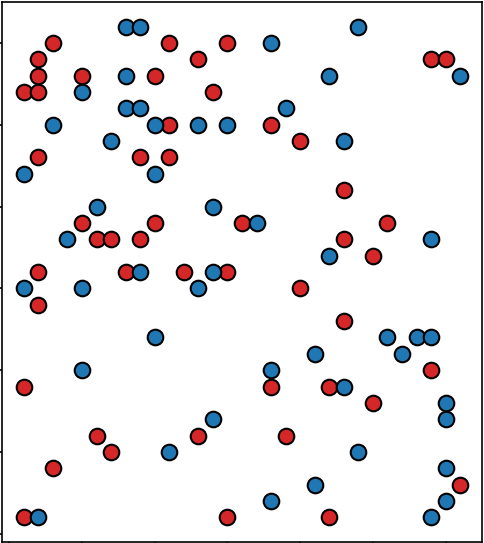
\includegraphics[width=0.5\linewidth]{Random_Inizialization.png}
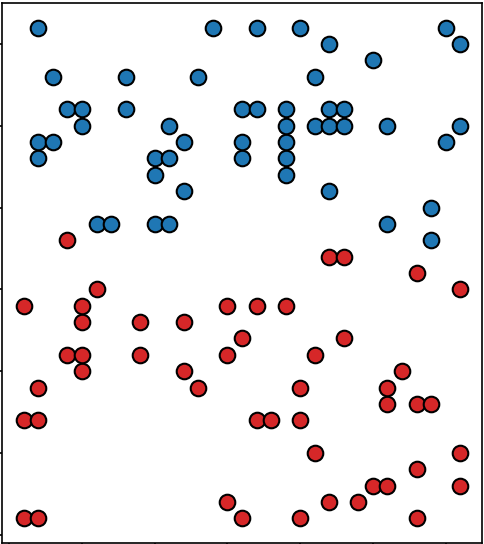
\includegraphics[width=0.5\linewidth]{Fixed_Inizialization.png}}
\par}
\caption{\textit{Esempio di due simulazioni con differenti modalità di inizializzazione: randomica a sinistra, ed ordinata a destra. }}
\label{Fig:12}
\end{figure}

Ripetendo fedelmente l'analisi descritta all'inizio, si è potuto constatare che tutte le stime dei parametri del fit a tangente iperbolica (nella tabella a seguire) sono risultate compatibili a quelle del caso precedente, ad eccezione di \textit{k} che ha riscontrato una diminuizione di un'ordine di grandezza.

\begin{center}
\begin{tabular}{ |c|c|c|c| } 
\hline
\ Parametri \ & \ Fit su "Tutti +1" \ & \ Fit su "Tutti -1" \ \\
\hline
\multirow{4}{4em}{\quad \textit{A} \\ \quad \textit{k} \\ \quad \textit{$\mu$} \\ \quad \textit{$\varphi$} } & -0.500 $\pm$ 0.002 & 0.500 $\pm$ 0.002 \\ 
& 4.8 $\pm$ 0.3 & 4.8 $\pm$ 0.3 \\ 
& -0.500 $\pm$ 0.004 & -0.500 $\pm$ 0.004 \\ 
& 0.506 $\pm$ 0.004 &  0.494 $\pm$ 0.004 \\
\hline
\end{tabular}
\end{center}

\begin{figure}[h]
\centering
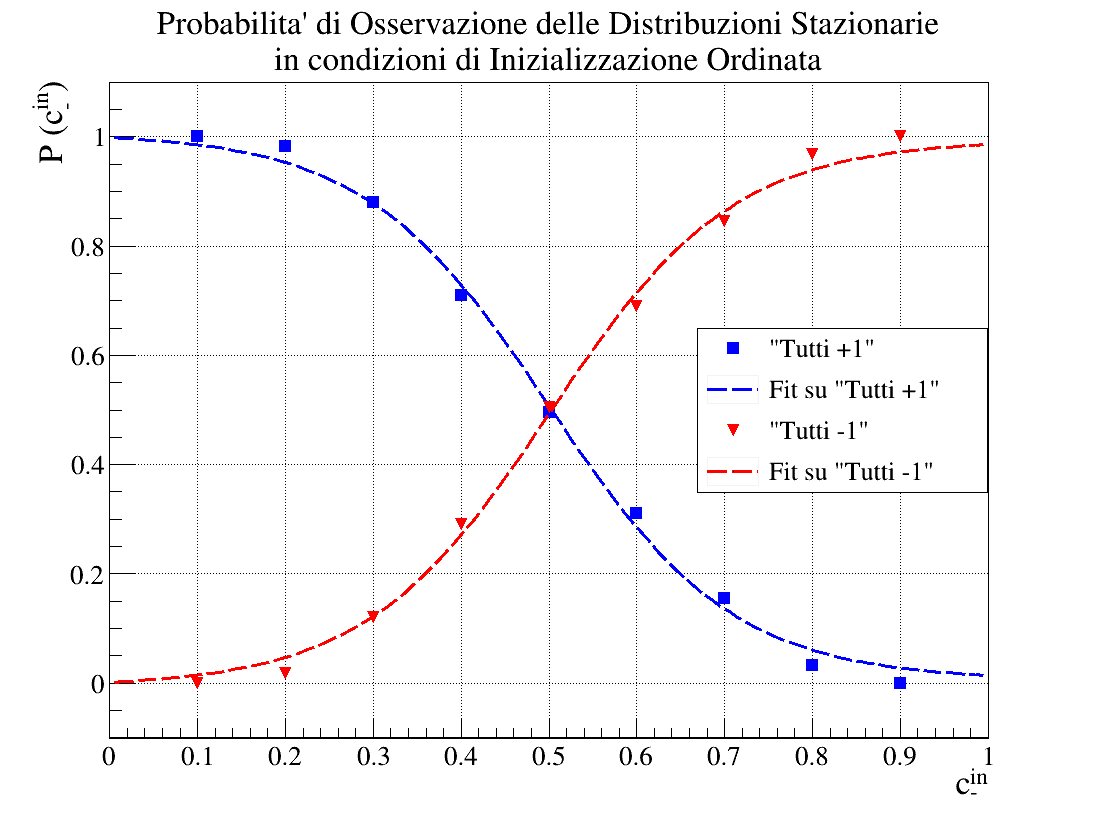
\includegraphics[width = \linewidth]{fixed_prob_graph.png}
\caption{\textit{bla bla bla}}
\label{Fig:9}
\end{figure}


\subsection{Visione Parziale}
\label{Sec:4.2}

\subsection{Flocking Gravitazionale}
\label{Sec:4.3}

Le regole di evoluzione della dinamica spaziale presentate nella Sezione \ref{Sec:3.3} hanno effetti notevoli sulla dinamica delle opinioni in quanto le due fazioni corrispondenti ai due stati $\pm1$ intraprendono una specie di ''guerra di logoramento'' in cui gli individui si dispongono in ''trincee'' e cercano di far prevalere la propria opinione (Vedi Fig.\ref{Fig:9}). 
\begin{figure}[h]
\centering
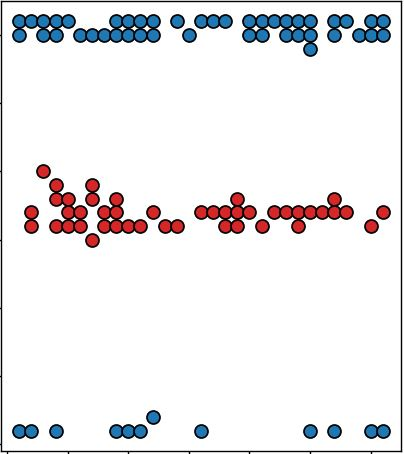
\includegraphics{trincea.jpg}
\caption{\textit{Configurazione caratteristica degli individui in una dinamica di flocking gravitazionale.}}
\label{Fig:9}

\end{figure}

Gli individui nei nuclei di queste trincee, che sono protetti dai vicini della stessa opinione, sono chiaramente difficili da conquistare mentre le parti più esterne, corrispondenti agli individui che si devono ancora aggregare al gruppo, sono più vulnerabili al cambio di opinione. La fine della guerra corrisponde a quando una delle due fazioni ha influenzato tutti gli individui dell'altra fazione, con il conseguente risultato di una distribuzione di opinioni omogenea corrispondente ad una condizione di equilibrio stabile. \\
Il raggiungimento di una delle due possibili condizioni stazionarie è fortemente dipendente dal parametro distanza di influenza $\delta$,  in particolare la dinamica è tanto più rapida quanto è maggiore il valore di $\delta$. Gli esempi riportati in figura \ref{Fig:10} portano una dimostrazione di quanto affermato attraverso l'analisi delle magnetizzazioni M(t).\\\\

L'analisi dei tempi di decisione $\tau$ ha manifestato un andamento a potenza come mostrato dai \textit{fit} in Figura \ref{Fig:11} eseguiti tramite la funzione introdotta nella Eq.\ref{Eq:11}. Le stime dei coefficienti \textit{c} e \textit{a} sono presentate nella seguente Tabella.

\begin{center}
\begin{tabular}{ |c|c|c|c| } 
\hline
 Simulazioni & \textit{c} & \textit{a} \\
\hline
\multirow{4}{4em}{$\delta$ = 1 \\$\delta$ = 2 \\$\delta$ = 4 \\$\delta$ = 8 }
& 0.182 $\pm$ 0.007 & -1.09 $\pm$ 0.05 \\ 
& 0.394 $\pm$ 0.011 & -1.68 $\pm$ 0.08 \\ 
& 0.265 $\pm$ 0.005 & -1.54 $\pm$ 0.05 \\ 
& 0.182 $\pm$ 0.007 &  -1.09 $\pm$ 0.05 \\
\hline
\end{tabular}
\end{center}

\begin{figure}
\centering
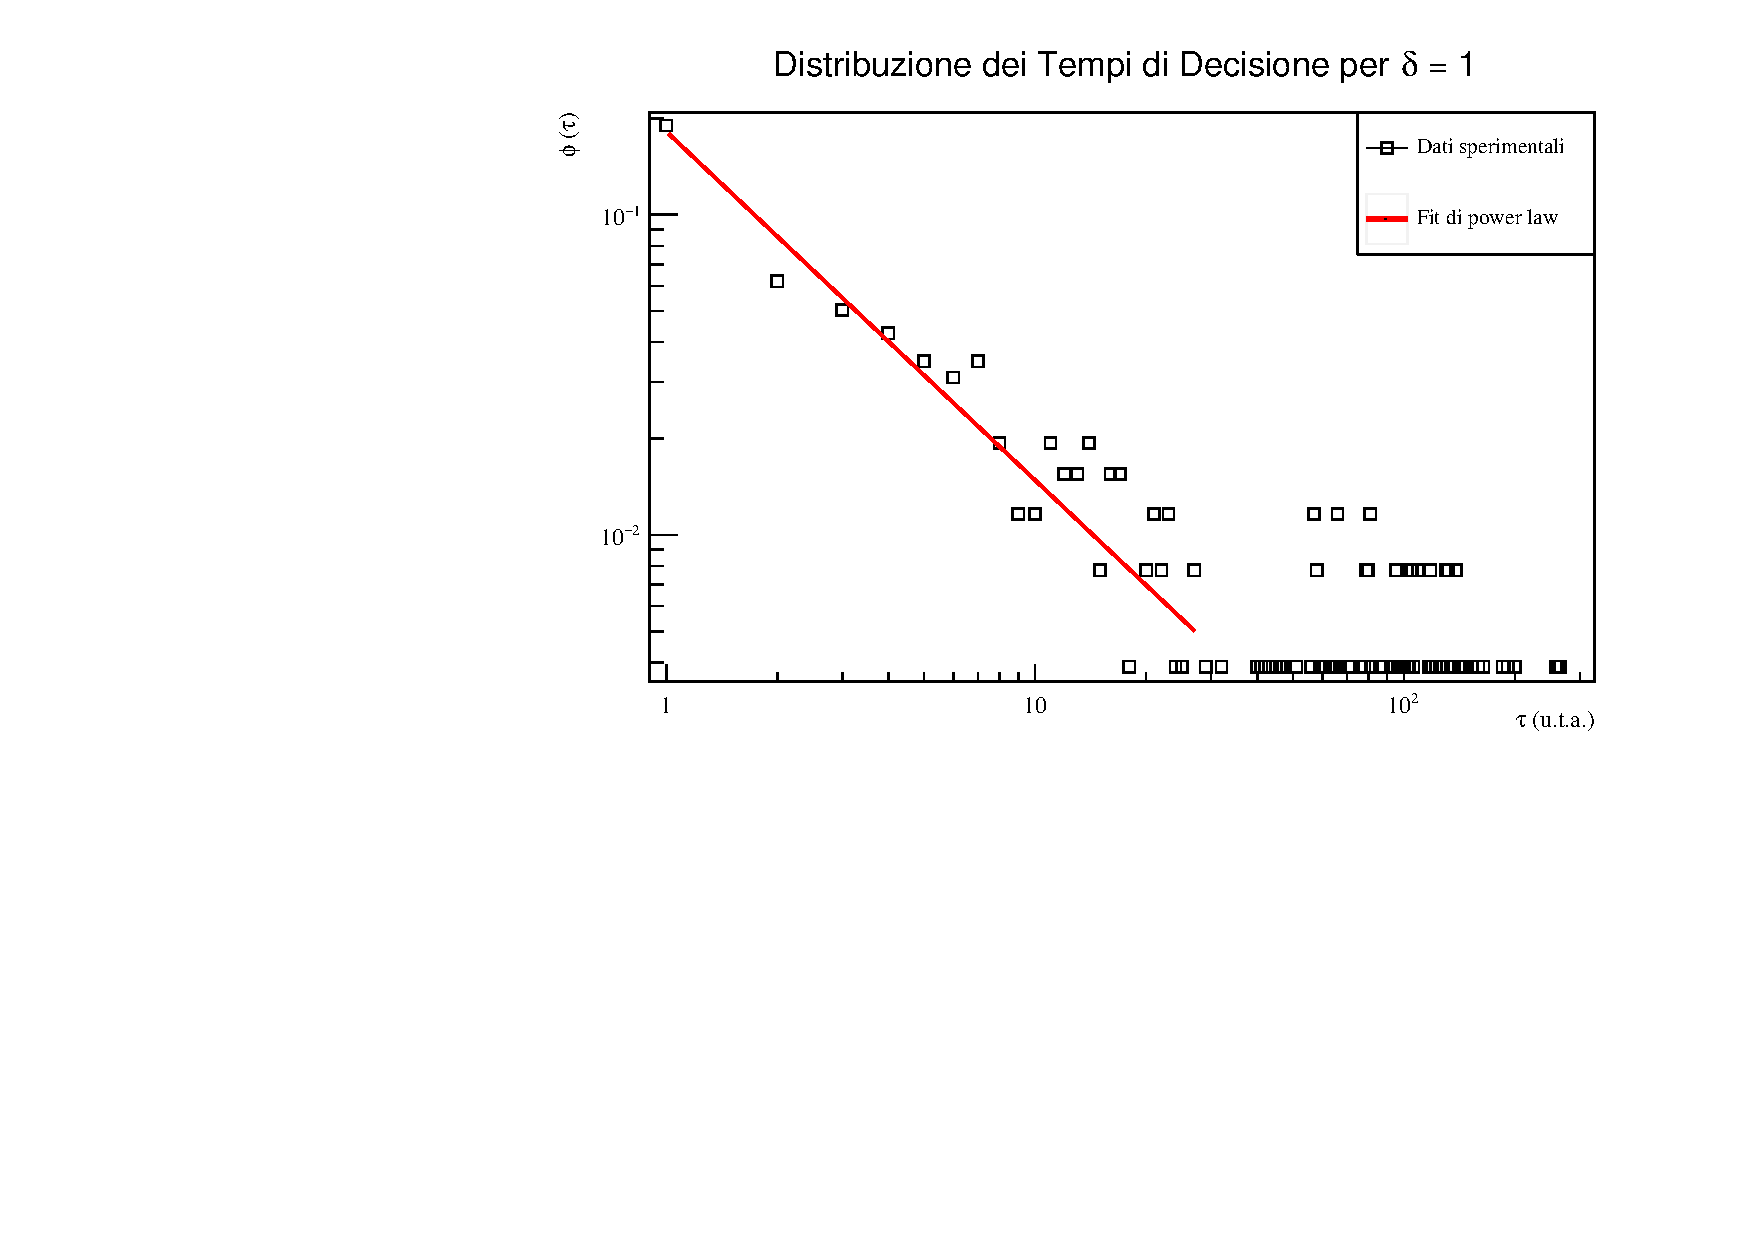
\includegraphics{tau1.pdf}
\end{figure}
\begin{figure}
\centering
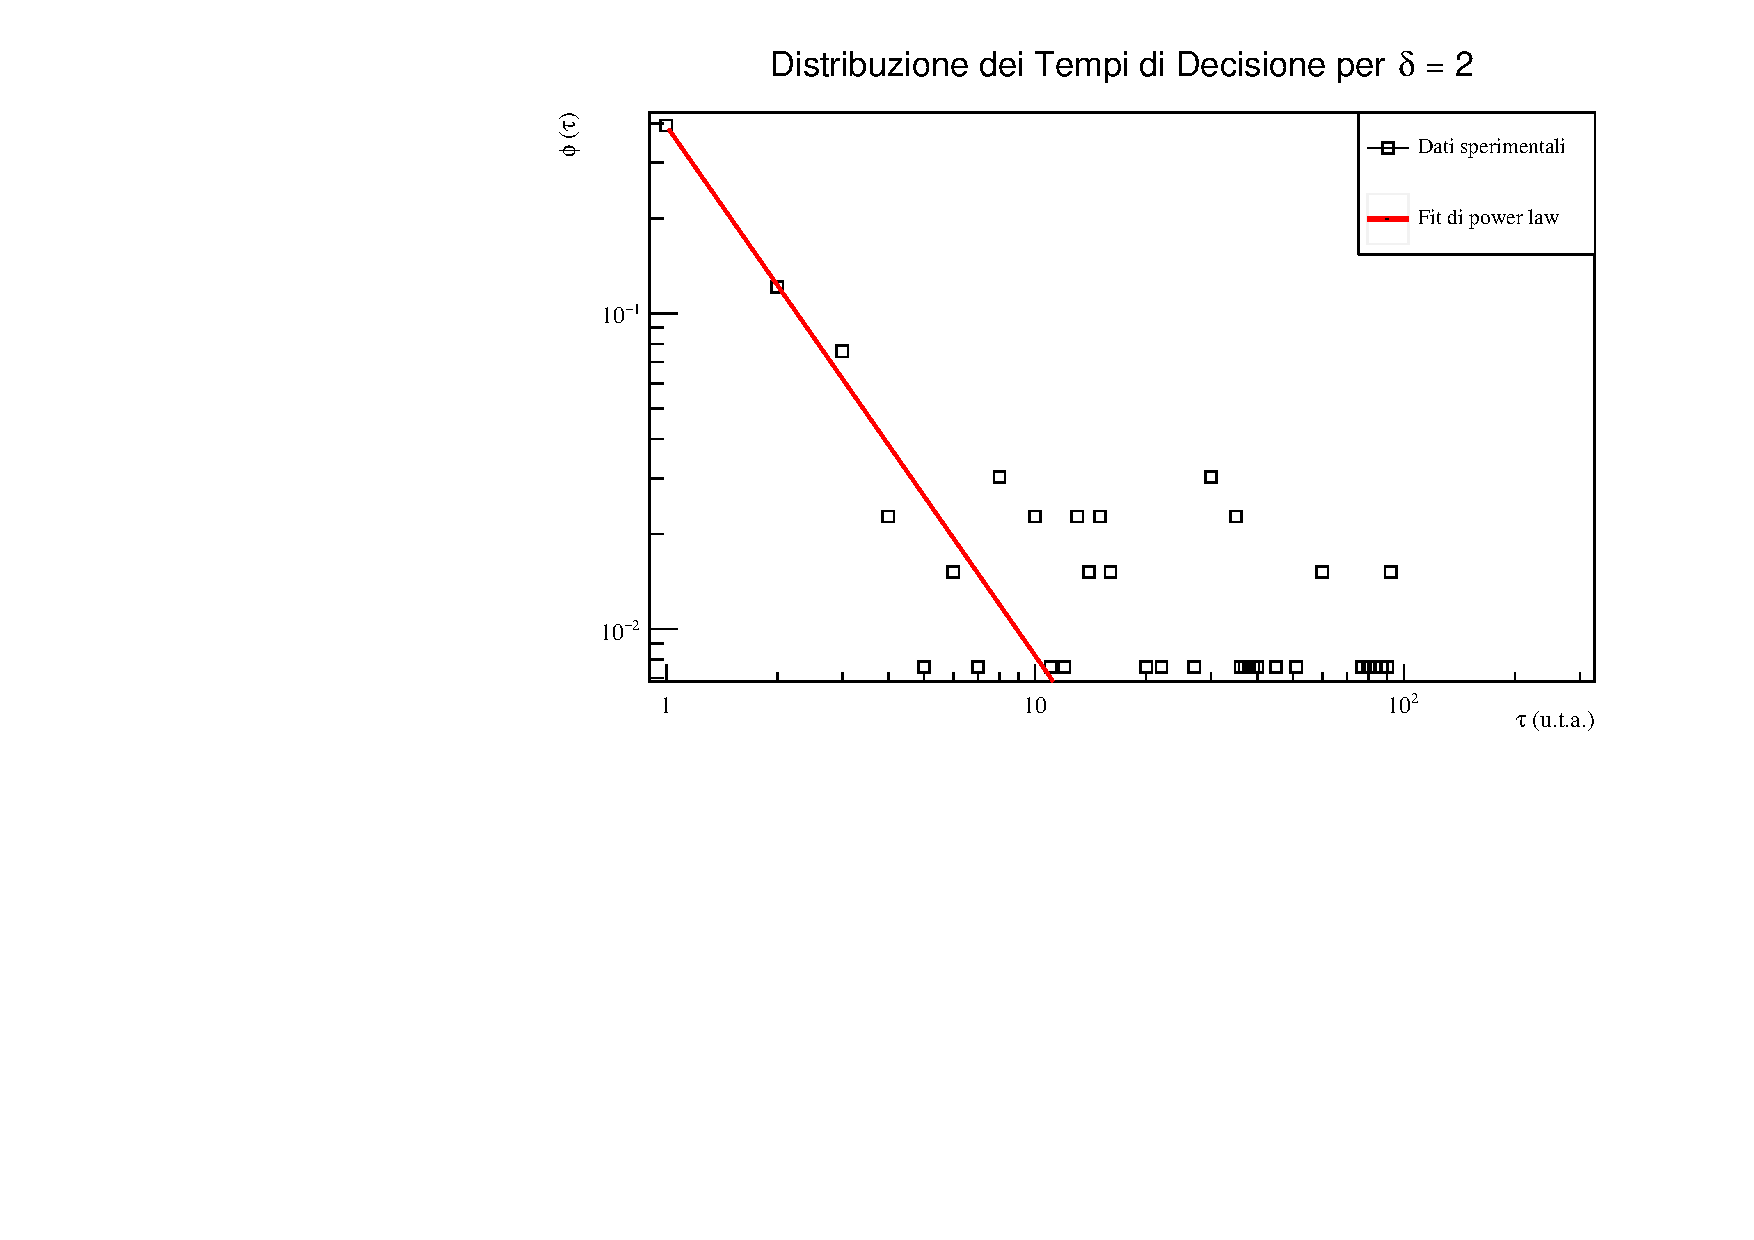
\includegraphics{tau2.pdf}
\end{figure}
\begin{figure}
\centering
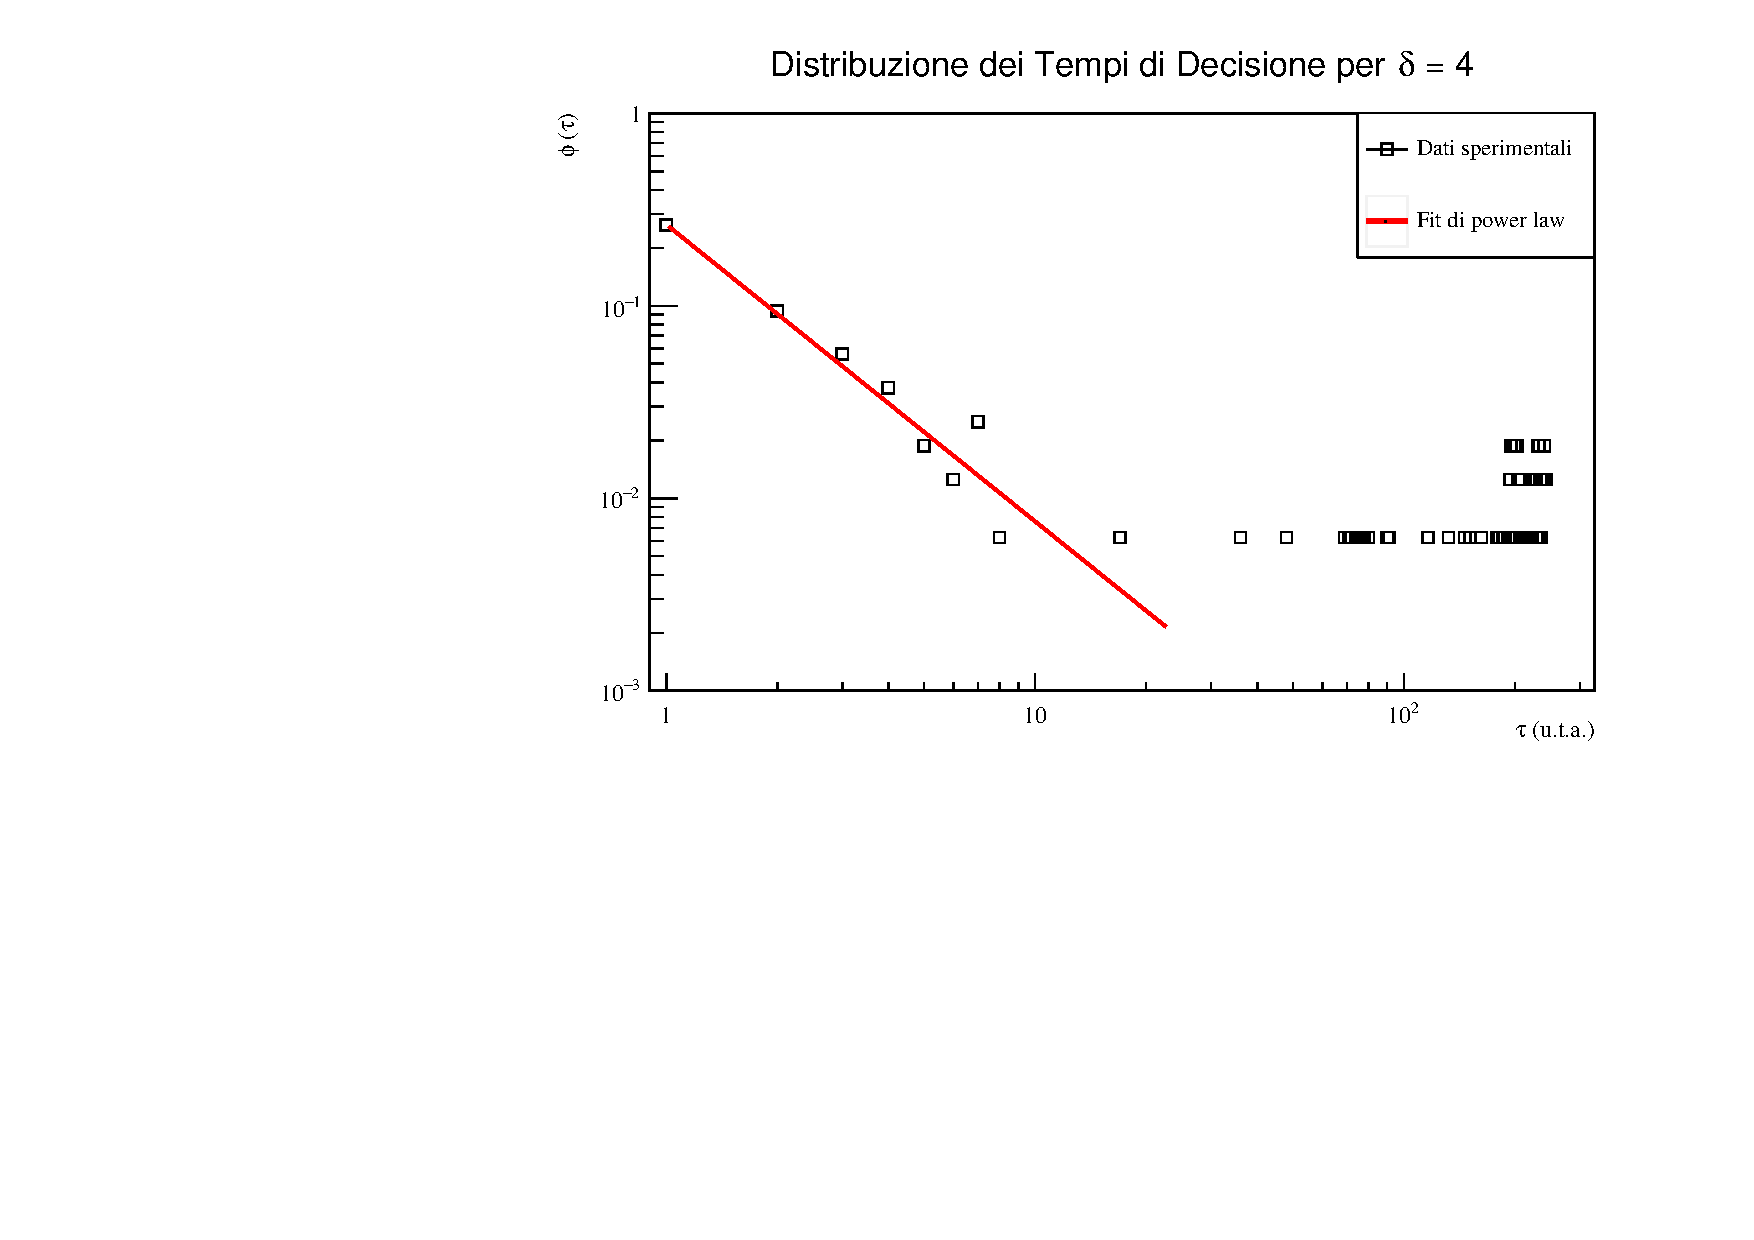
\includegraphics{tau4.pdf}
\end{figure}
\begin{figure}
\centering
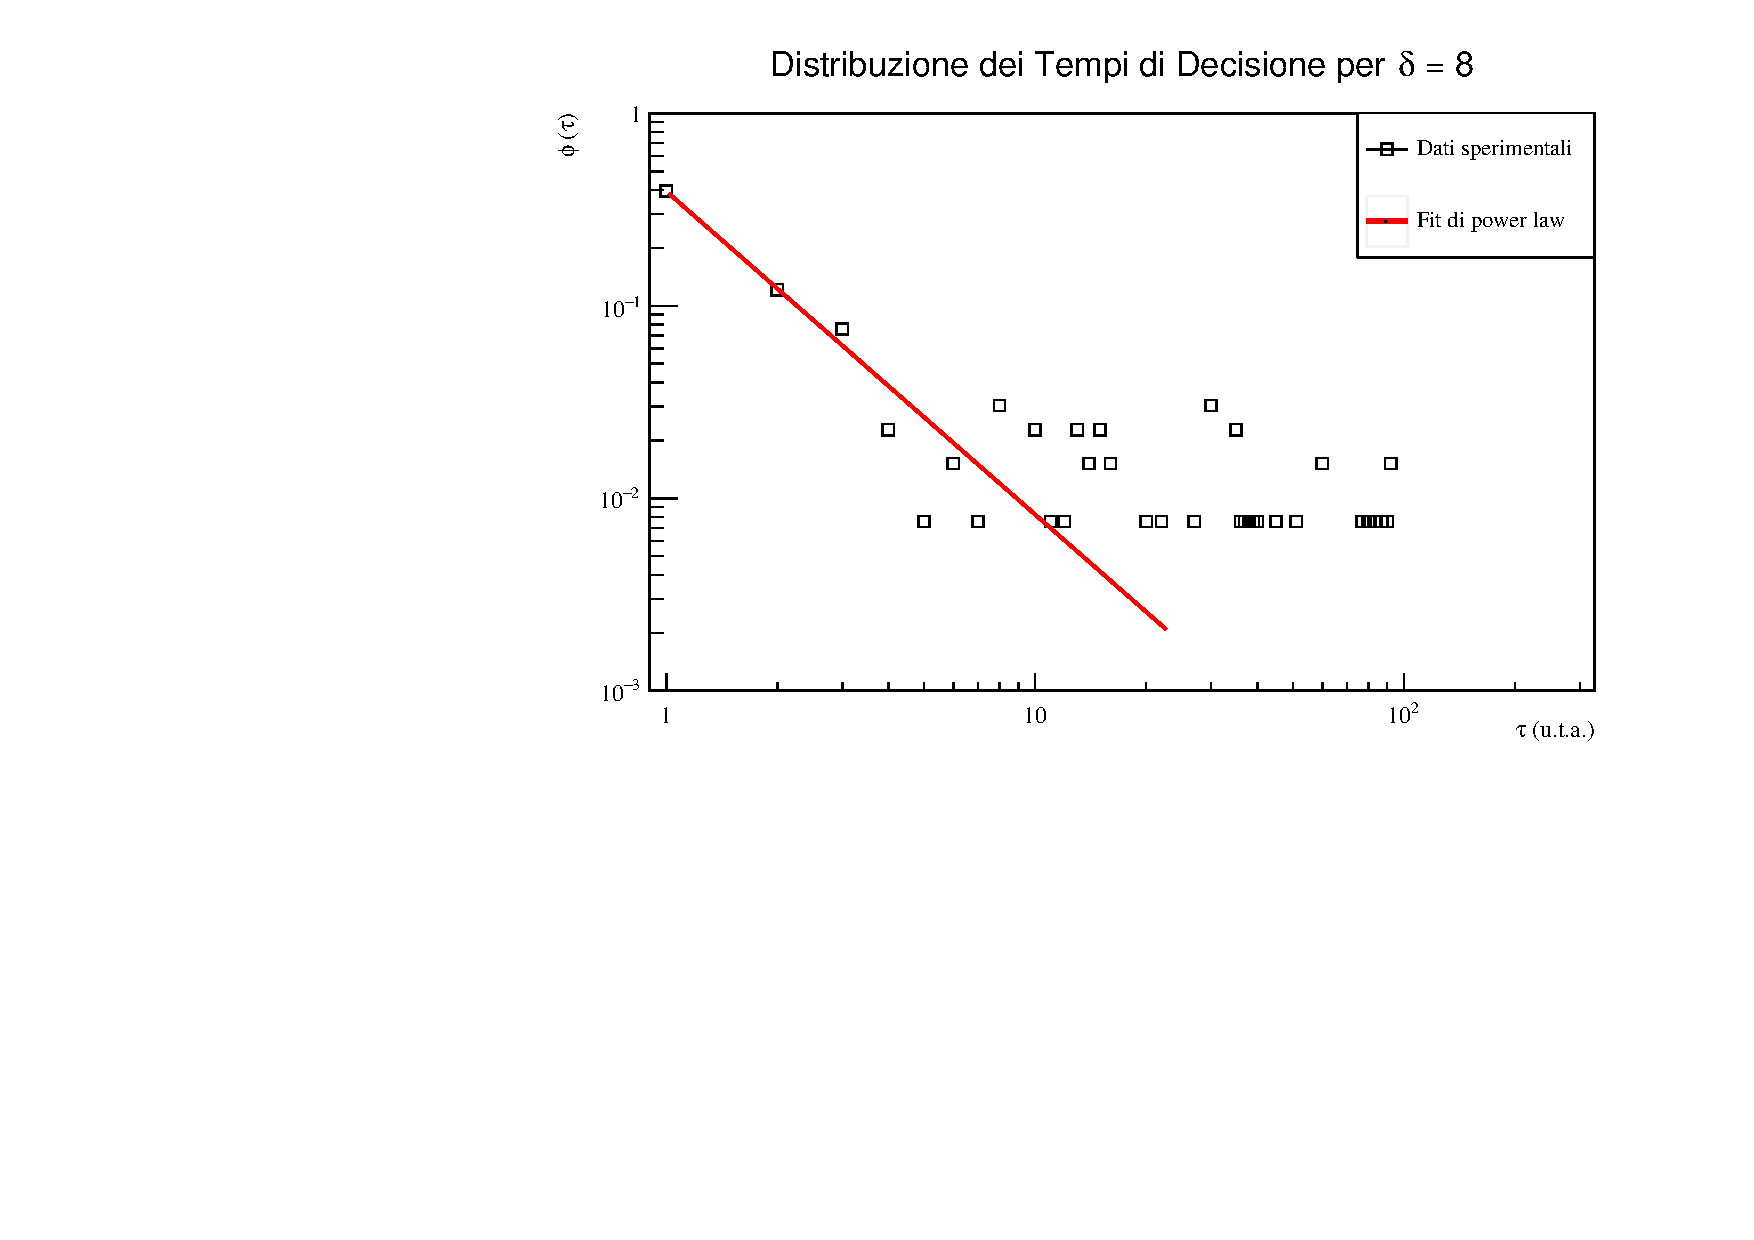
\includegraphics{tau8.pdf}
\end{figure}

È interessante notare che in questo tipo di modello, per come è costruita la dinamica degli individui, il raggiungimento di una condizione di equilibrio stabile può richiedere un numero di step temporali di simulazione molto elevato. Qui di seguito è stato riportato un esempio in cui si sono studiati la magnetizzazione
e i tempi di decisione degli individui in una simulazione durata \textit{10078 steps}.

\begin{figure}
\centering
\begin{subfigure}[h]{1.2\linewidth}
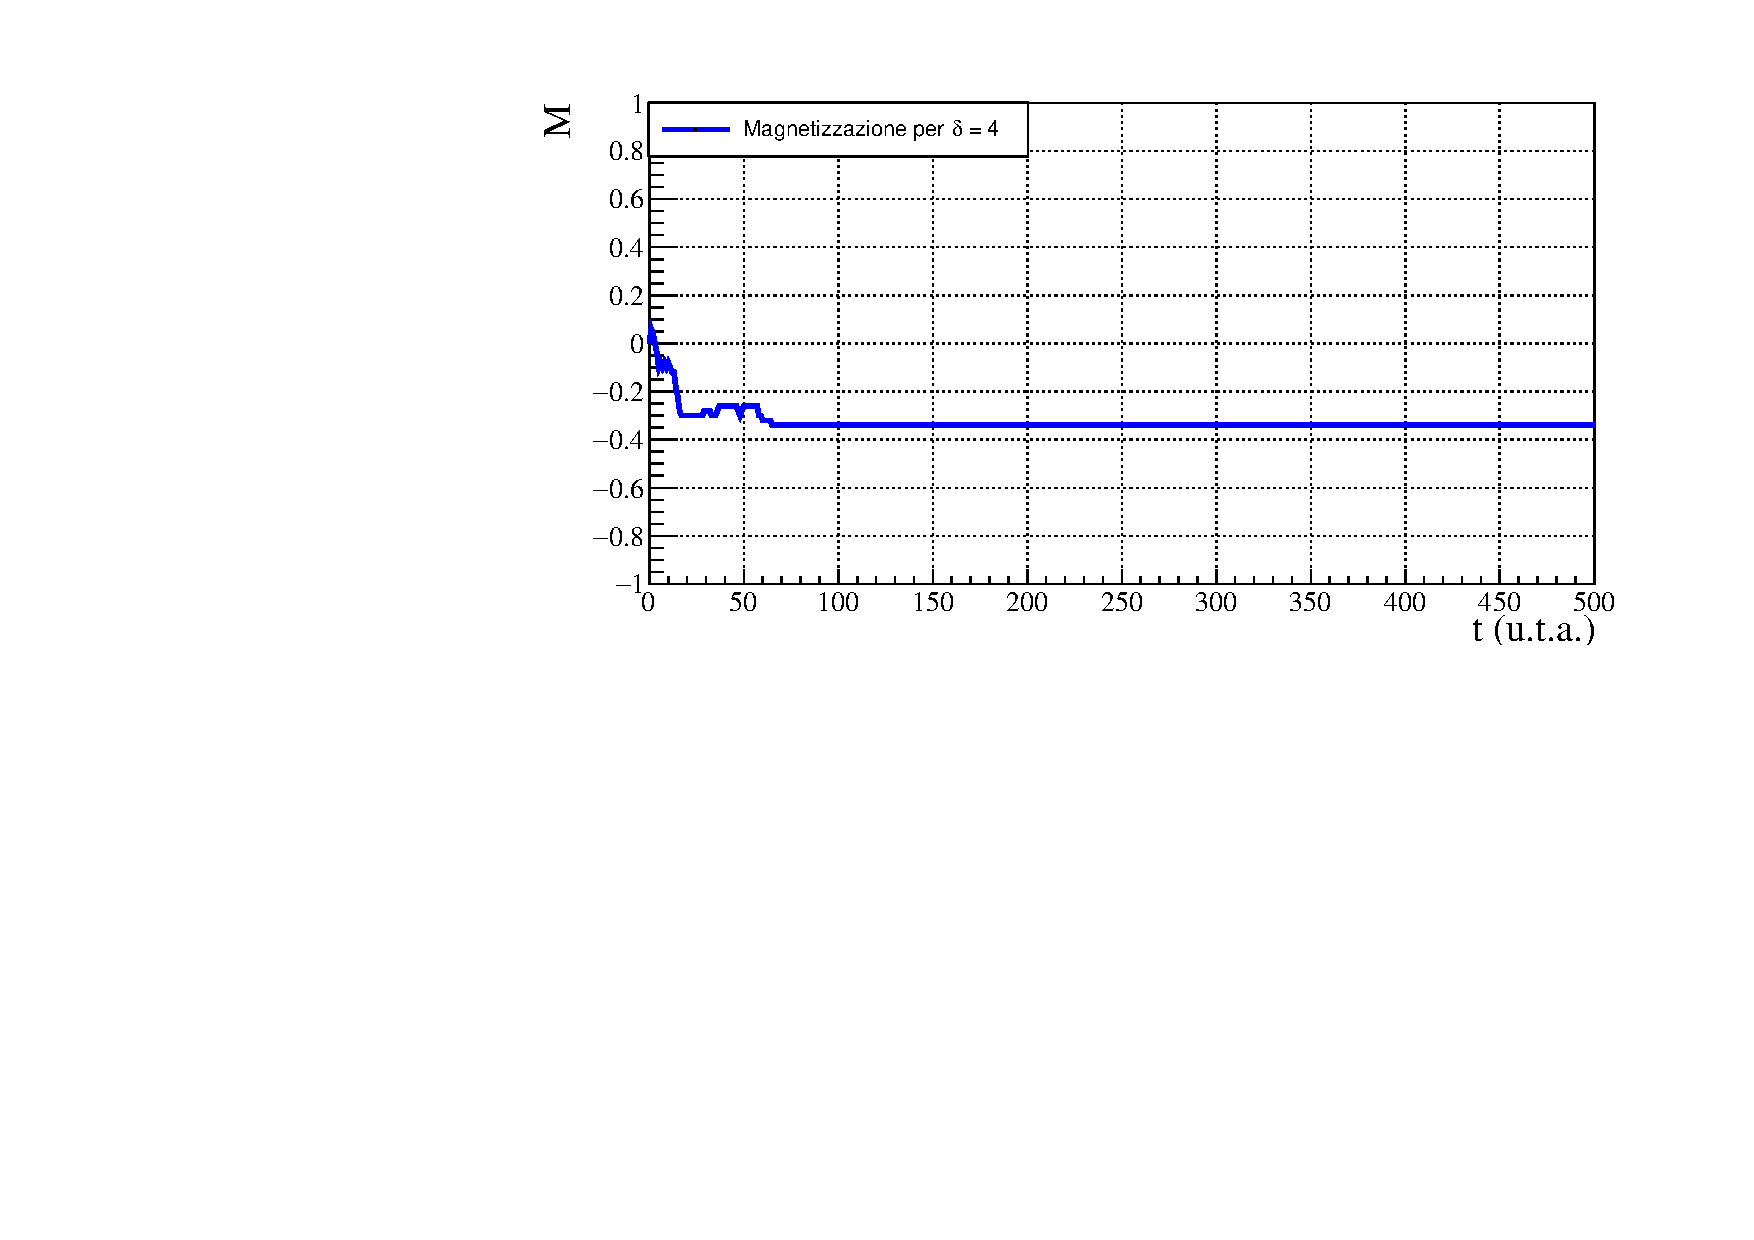
\includegraphics[width=\linewidth]{mag.pdf}
\end{subfigure}
\begin{subfigure}[h]{1.2\linewidth}
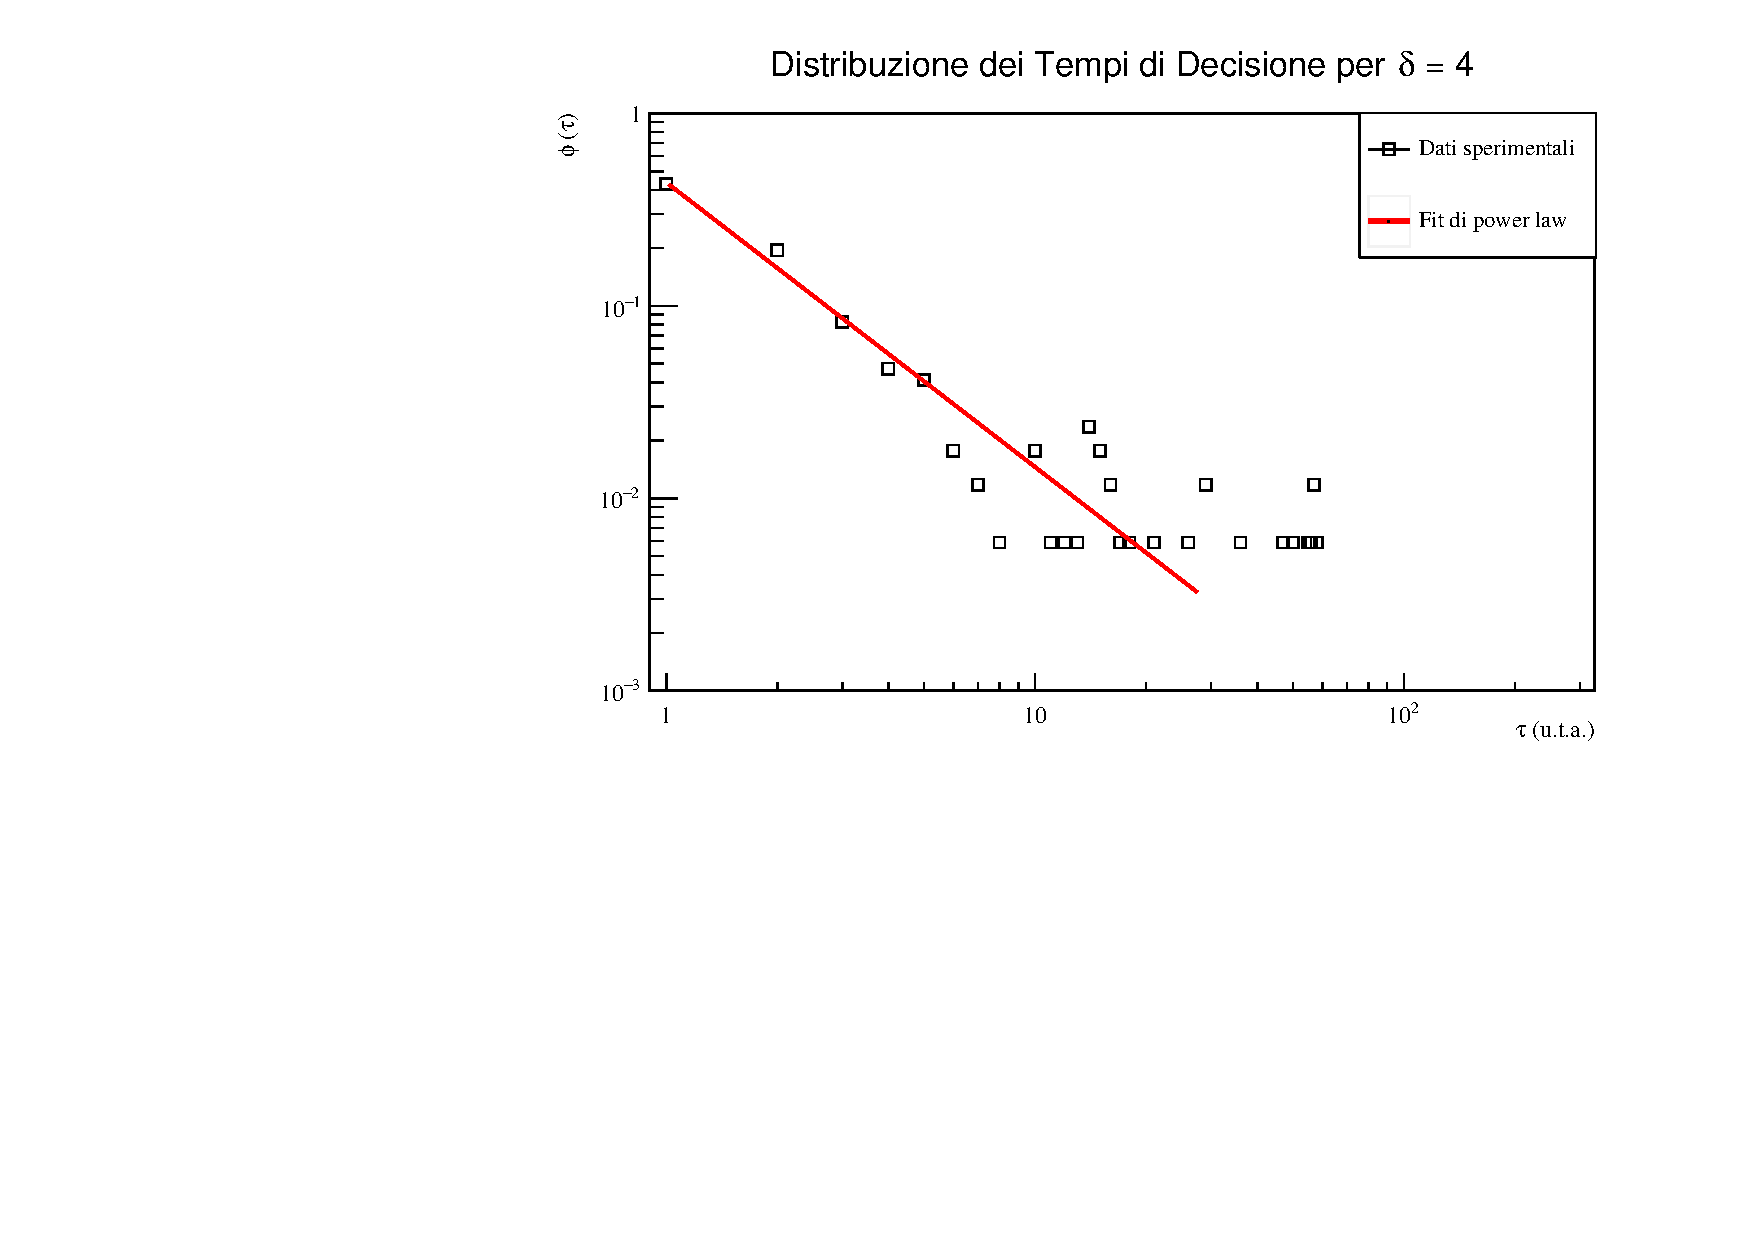
\includegraphics[width=\linewidth]{tau_10078.pdf}
\end{subfigure}
\label{Fig:13}
\end{figure}

La stima dei parametri di \textit{fit} del grafico in Figura \ref{Fig:13} sono i seguenti:

\begin{center}
\begin{tabular}{ |c|c|c|c| } 
\hline
 Simulazioni & \textit{c} & \textit{a} \\
\hline
\multirow{1}{3em}{$\delta$ = 4 }
& 0.438 $\pm$ 0.010 & -1.48 $\pm$ 0.05 \\ 
\hline
\end{tabular}
\end{center}.

Lo studio della influenza delle condizioni iniziali nella distribuzione di equilibrio del sistema è stato fatto su un campione di 500 simulazioni, eseguite variando la concentrazione $c^{in}_{ \_ }$ di agenti con opinione -1 ogni 100 esecuzioni della simulazione. Il risultato di questa analisi è graficato in Figura\ref{Fig:12}.

\begin{figure}
\centering
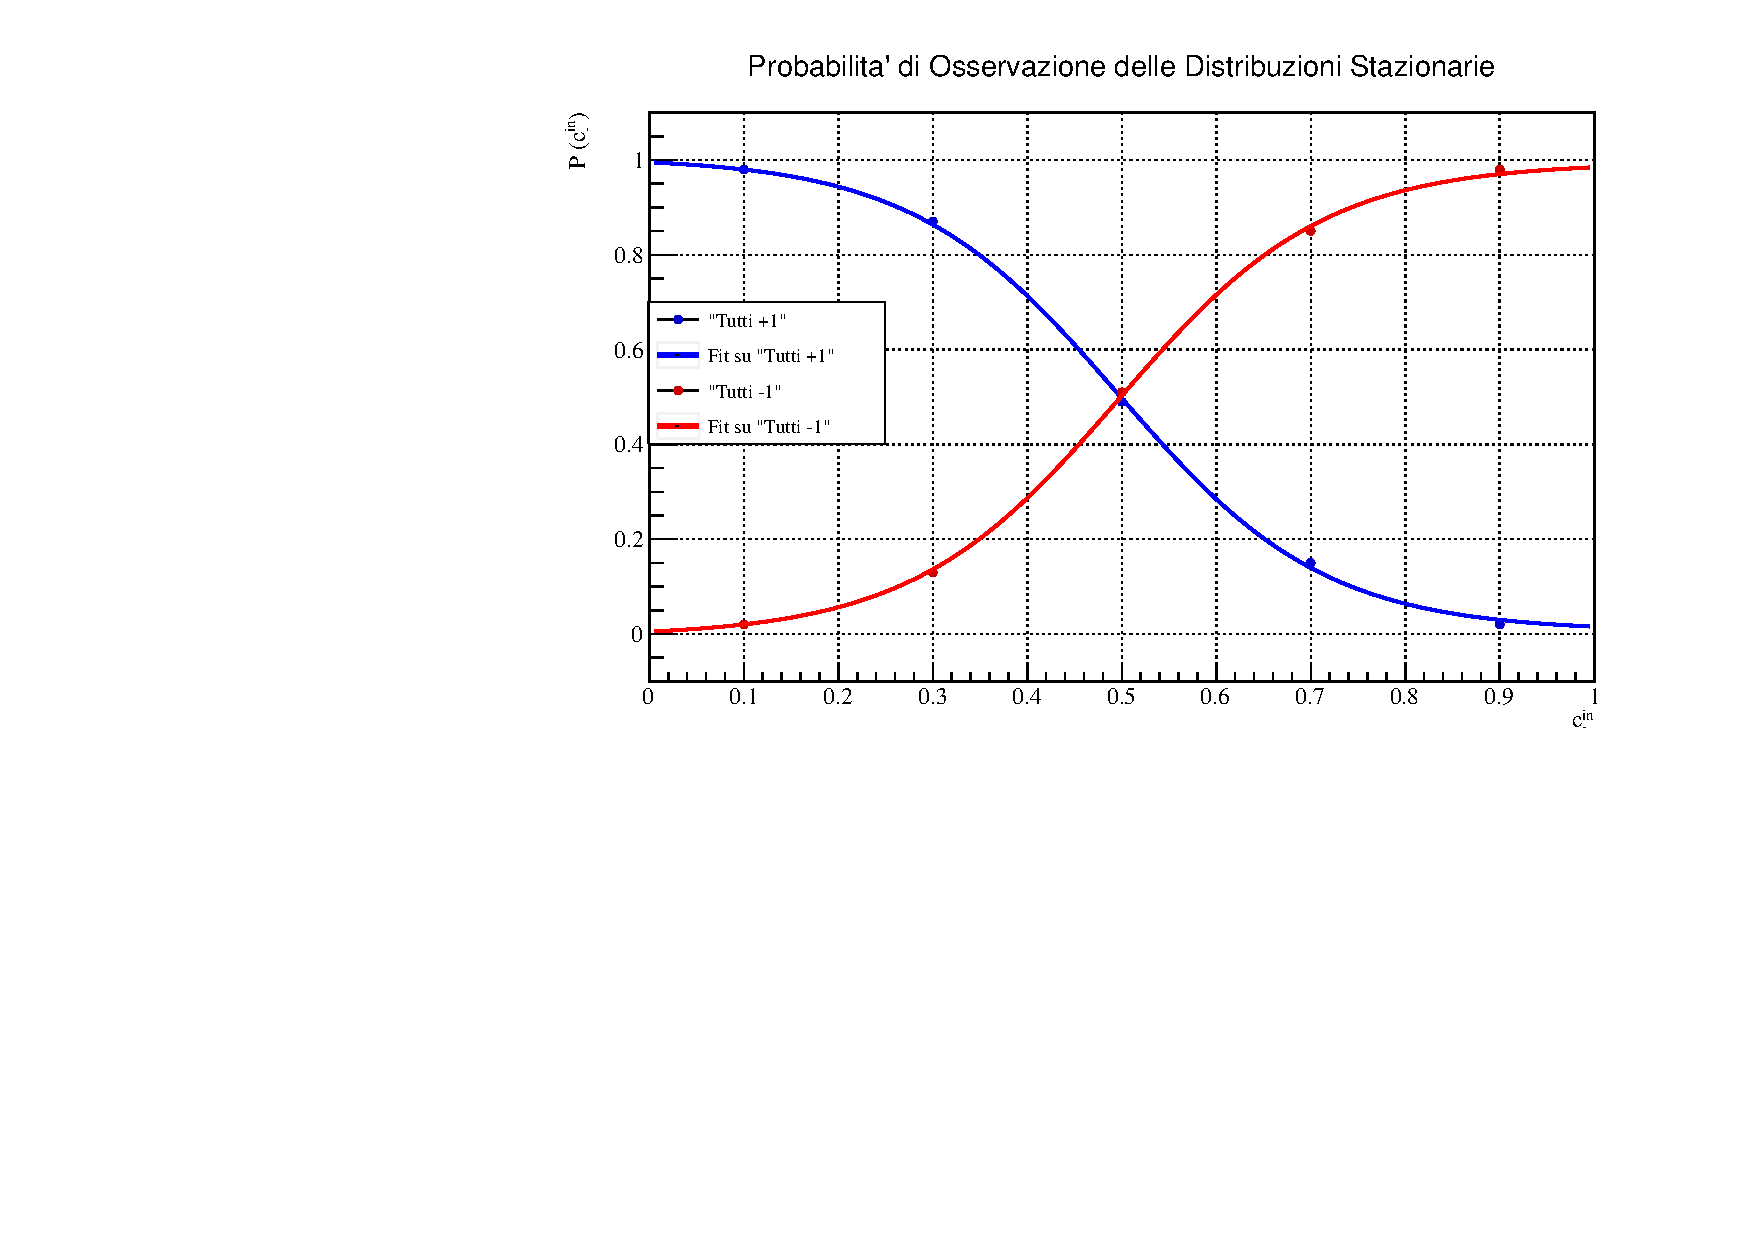
\includegraphics{fit_grav.pdf}
\label{Fig:12}
\end{figure}

I \textit{fit} dei dati sono stati eseguiti attraverso la tangente iperbolica in Eq.\ref{Eq:12} e hanno portato alla stima dei parametri di \textit{fit} riportati in Tabella.

\begin{center}
\begin{tabular}{ |c|c|c|c| } 
\hline
\ Parametri \ & \ Fit su "Tutti +1" \ & \ Fit su "Tutti -1" \ \\
\hline
\multirow{4}{4em}{\quad \textit{A} \\ \quad \textit{k} \\ \quad \textit{$\mu$} \\ \quad \textit{$\varphi$} } 
& -0.4999 $\pm$ 0.0004 & 0.4999 $\pm$ 0.0014 \\ 
& 4.586 $\pm$ 0.011 & 4.586 $\pm$ 0.009 \\ 
& -0.496 $\pm$ 0.003 & -0.496 $\pm$ 0.003 \\ 
& 0.506 $\pm$ 0.003 &  0.494 $\pm$ 0.002 \\
\hline
\end{tabular}
\end{center}
Il coefficiente di determinazione $R^2$ = 0.999587 è molto vicino al valore ottimale 1, ciò è un indice di bontà del \textit{fit}.

\begin{figure}
\centering
\begin{subfigure}[h]{1.2\linewidth}
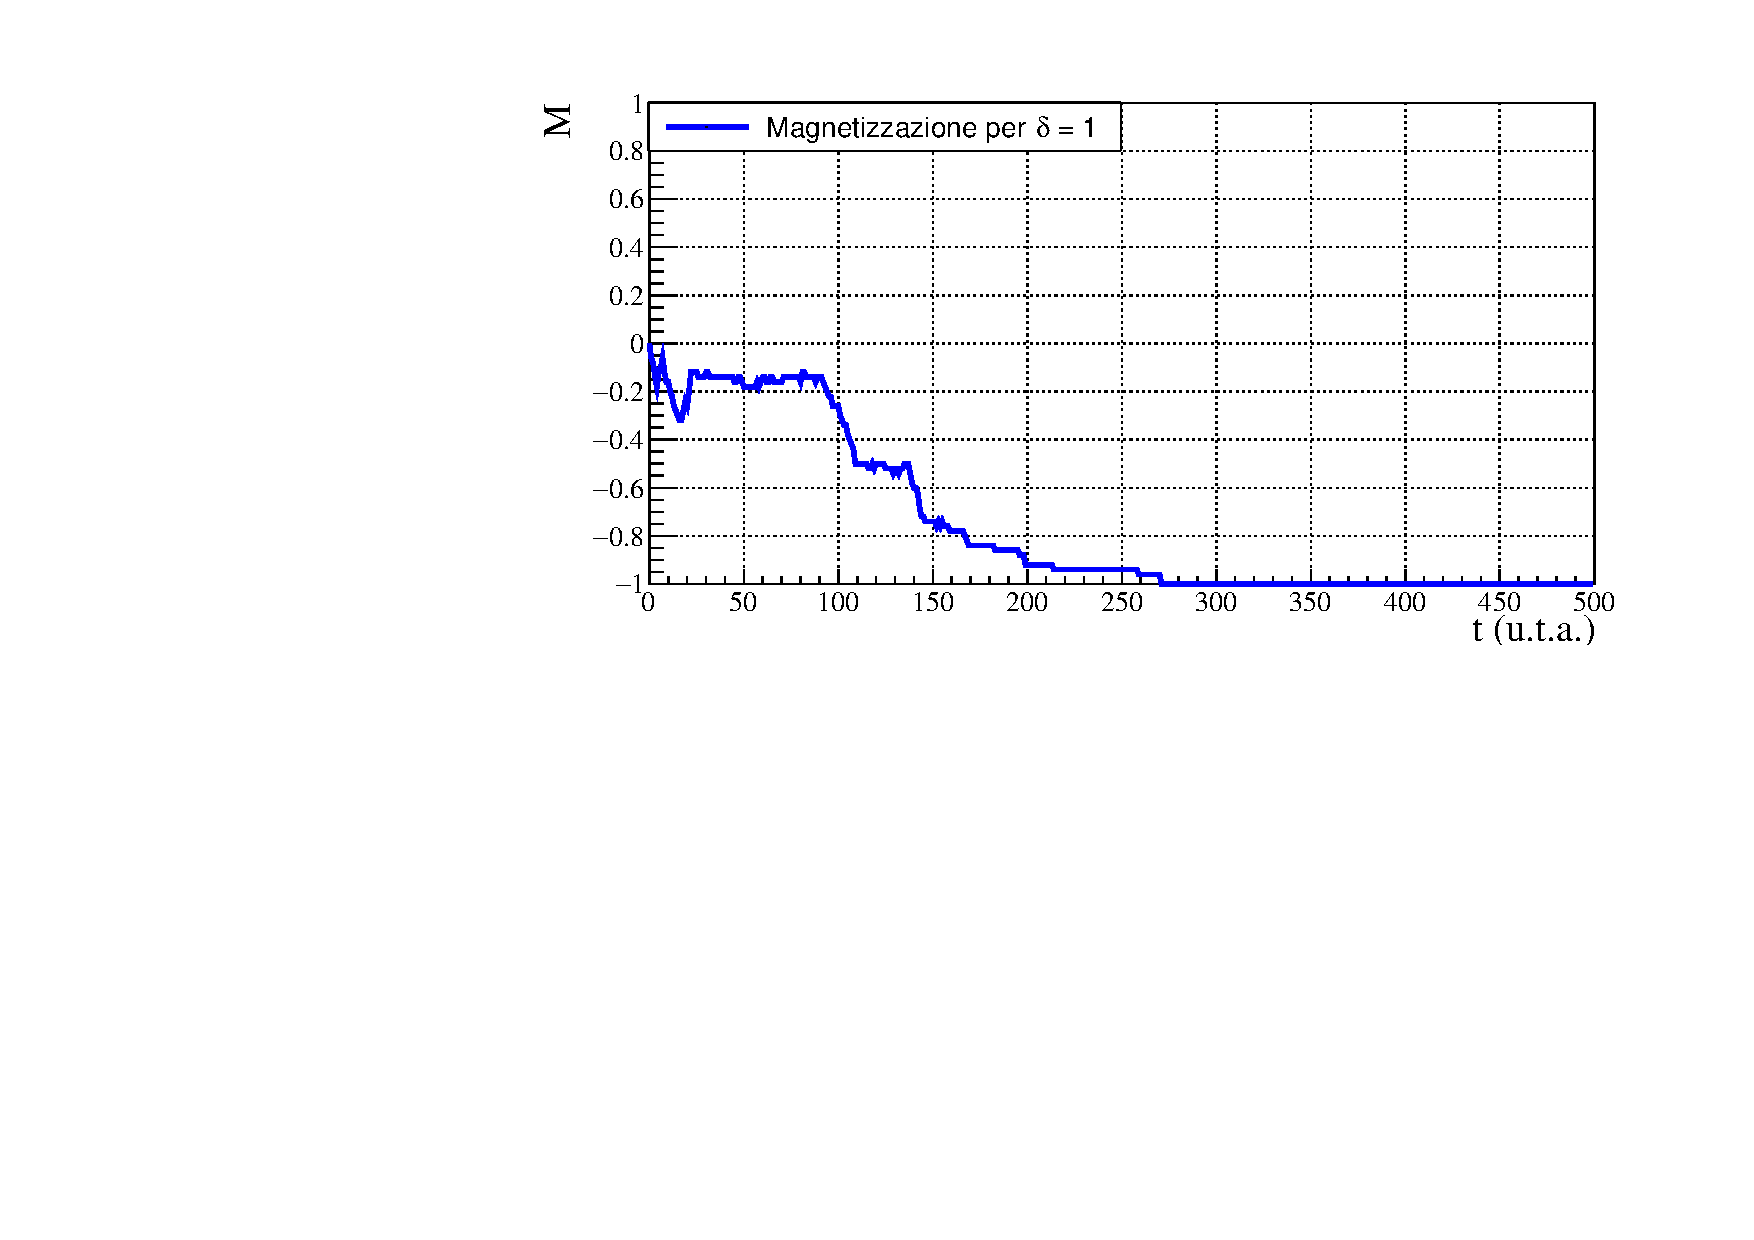
\includegraphics[width=\linewidth]{mag_d1.pdf}
\end{subfigure}
\begin{subfigure}[h]{1.2\linewidth}
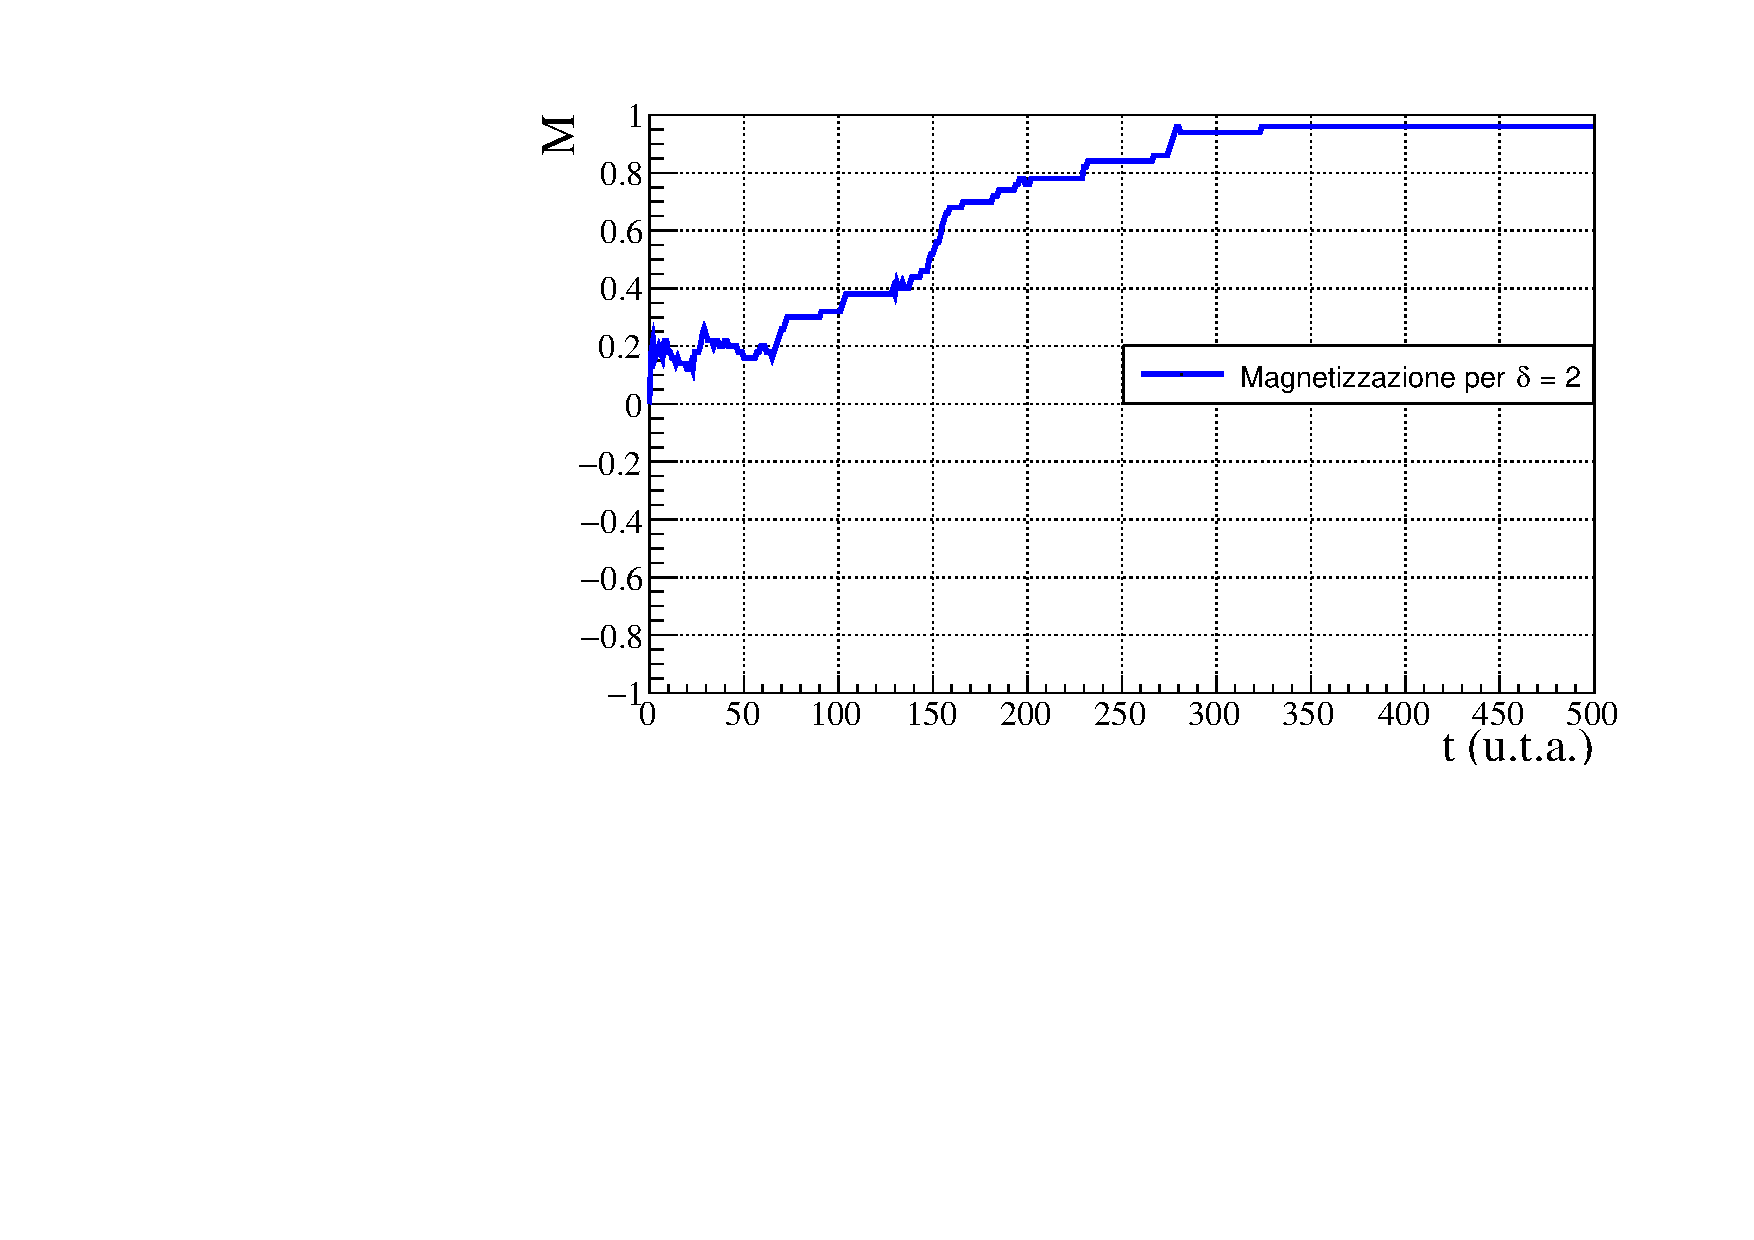
\includegraphics[width=\linewidth]{mag_d2.pdf}
\end{subfigure}
\end{figure}

\begin{figure}[h]
\centering
\begin{subfigure}[h]{1.2\linewidth}
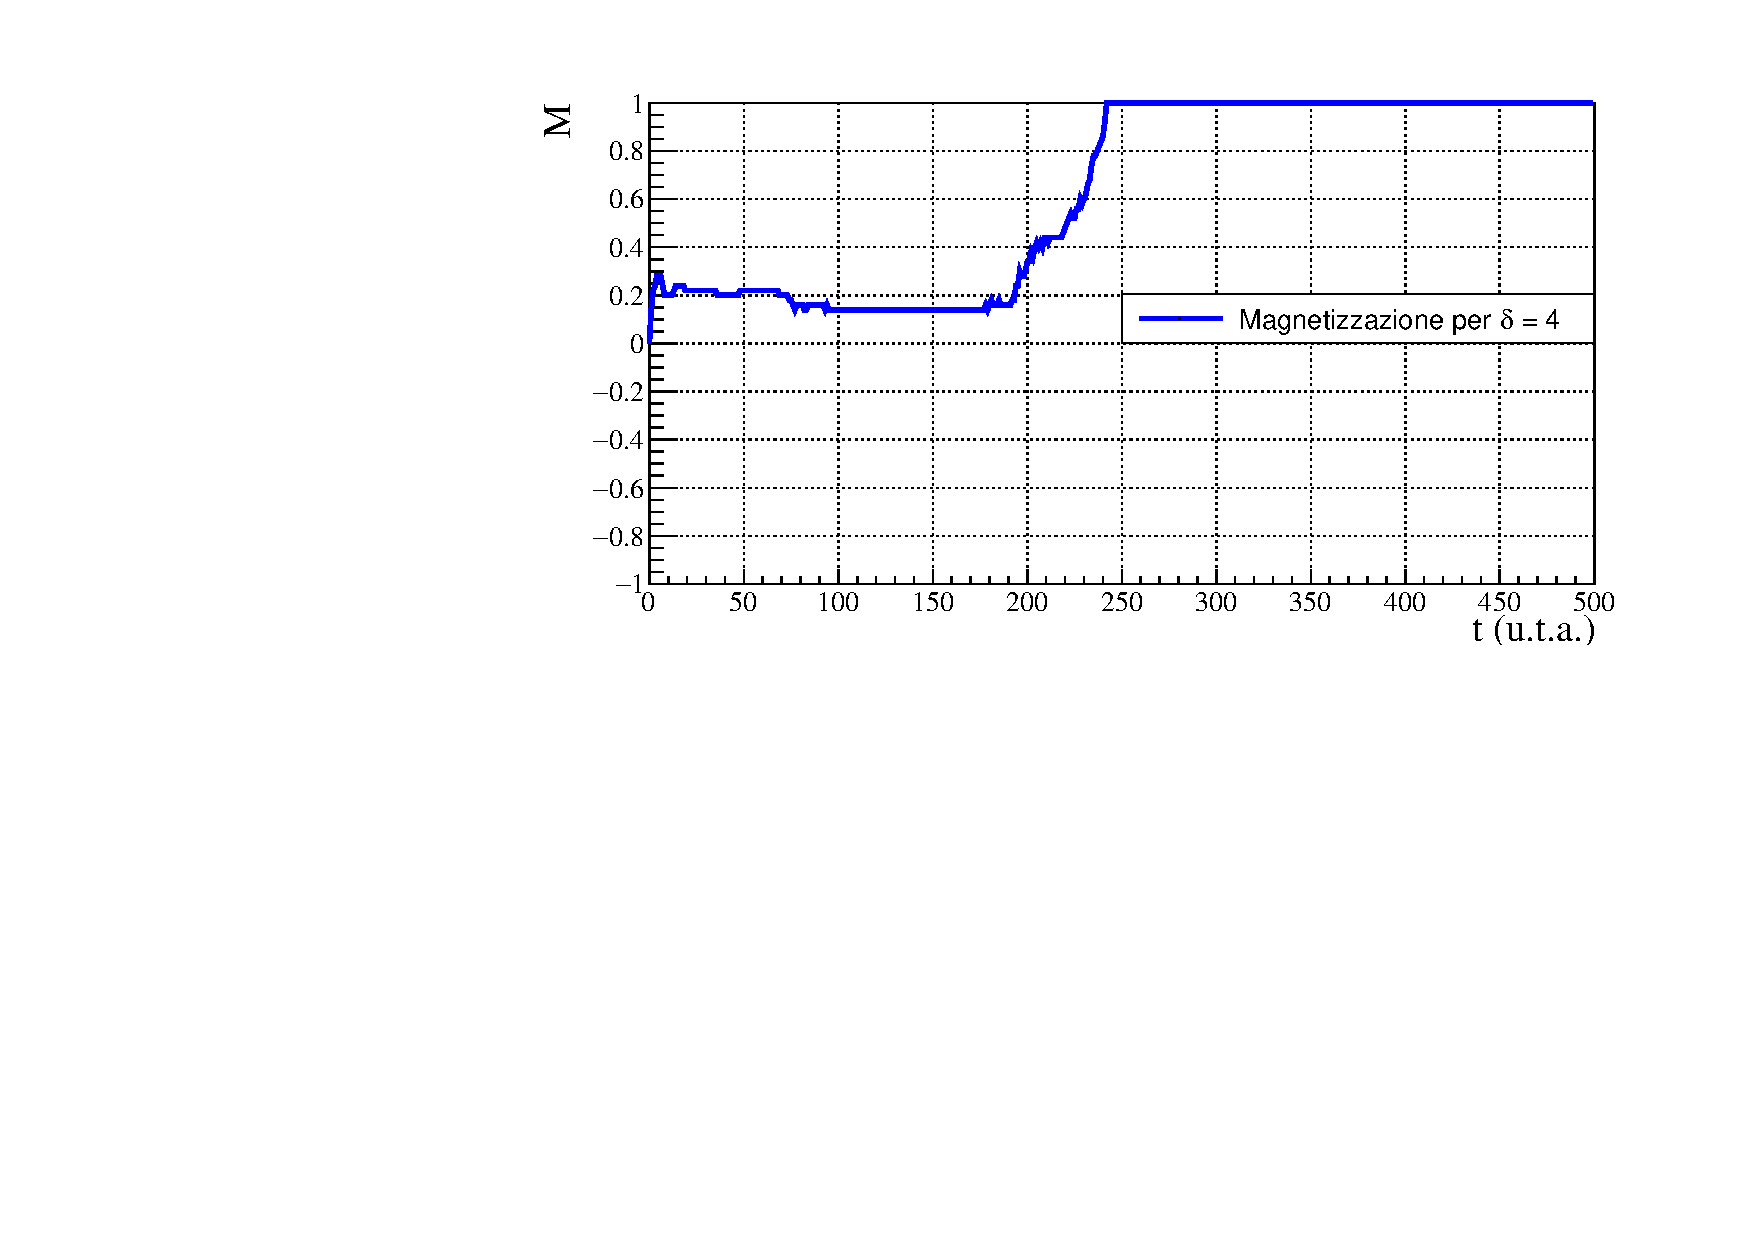
\includegraphics[width=\linewidth]{mag_d4.pdf}
\end{subfigure}
\begin{subfigure}[h]{1.2\linewidth}
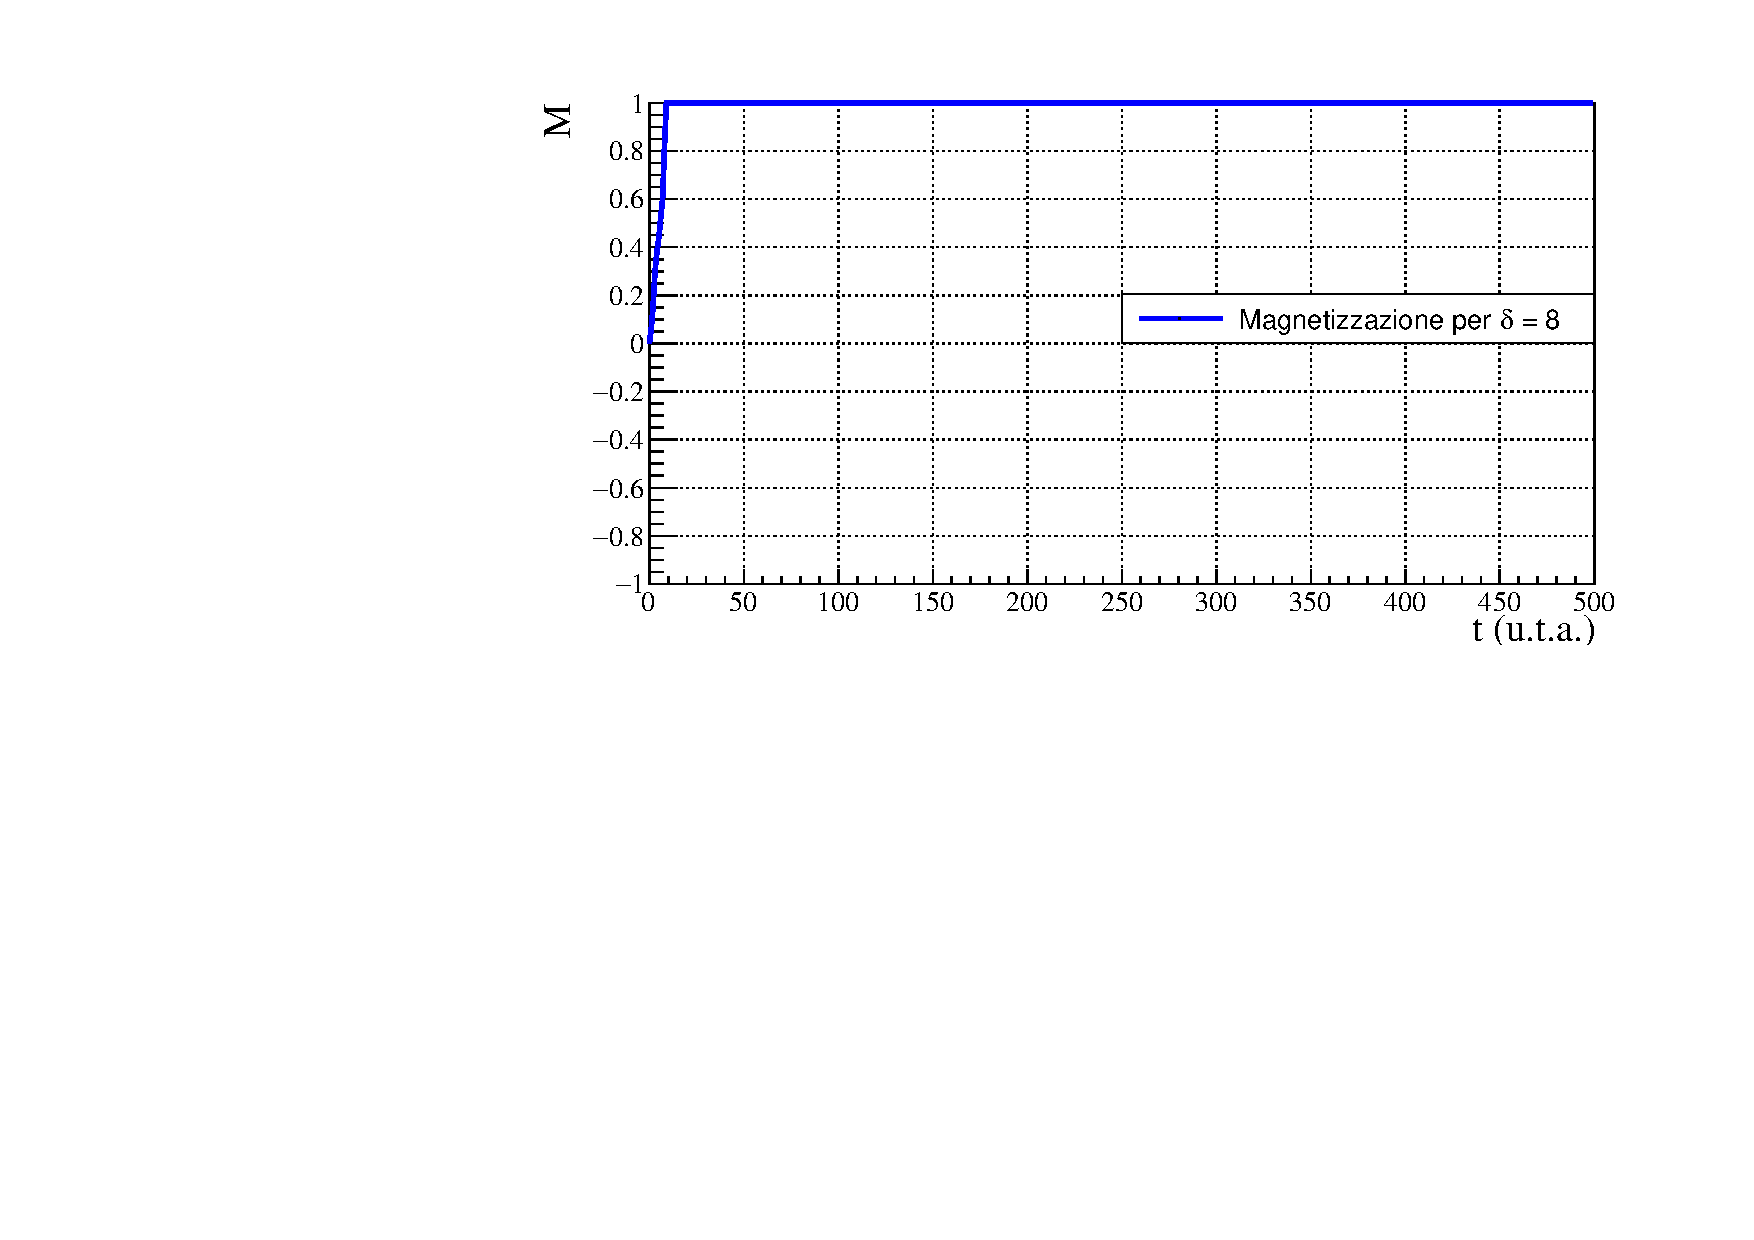
\includegraphics[width=\linewidth]{mag_d8.pdf}
\end{subfigure}

\label{Fig:10}
\caption{SUUUU }
\end{figure}



\subsection{Confronto ai Dati}
\label{Sec:4.5}

\begin{figure}[h]
\centering
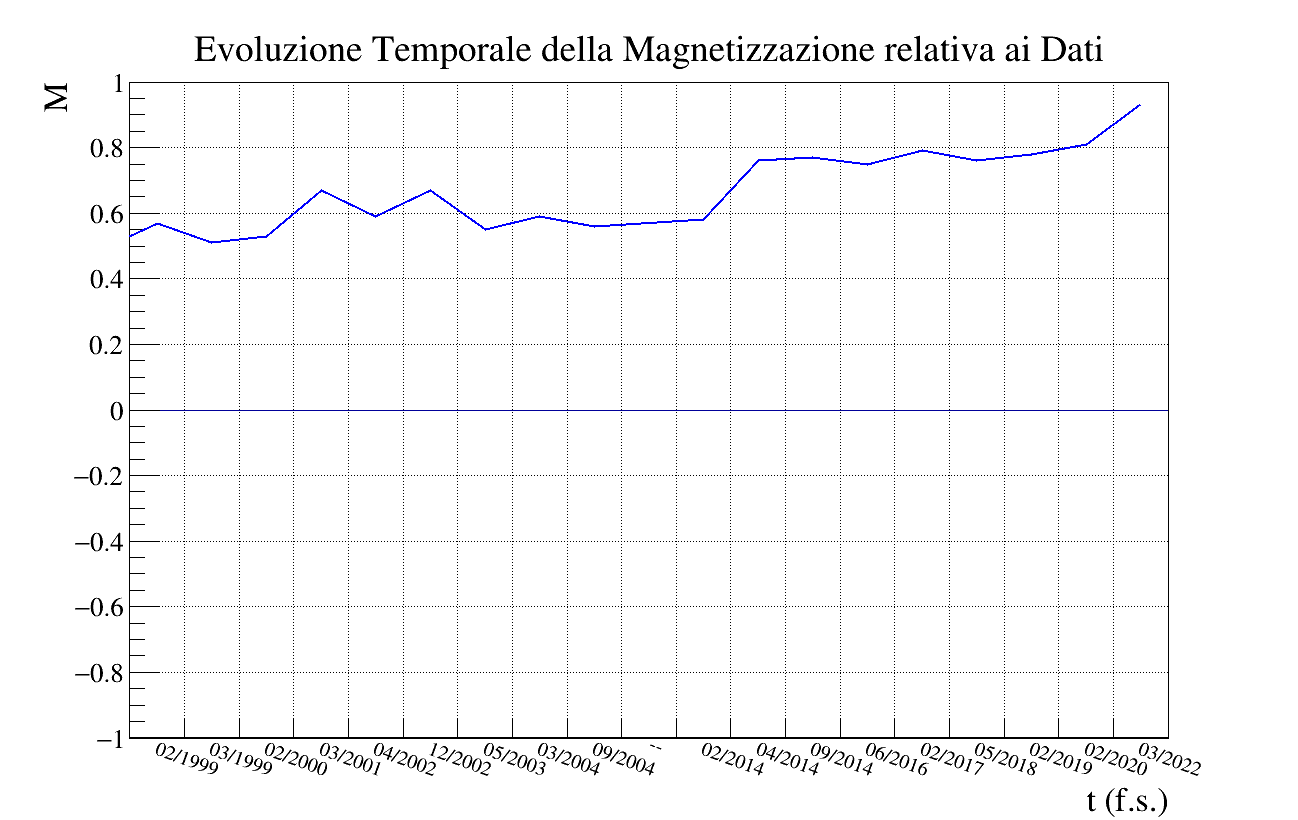
\includegraphics[width = 1.1\linewidth]{poland_magnetization_graph.png}
\caption{\textit{bla bla bla}}
\label{Fig:9}
\end{figure}

\begin{figure}[h]
\centering
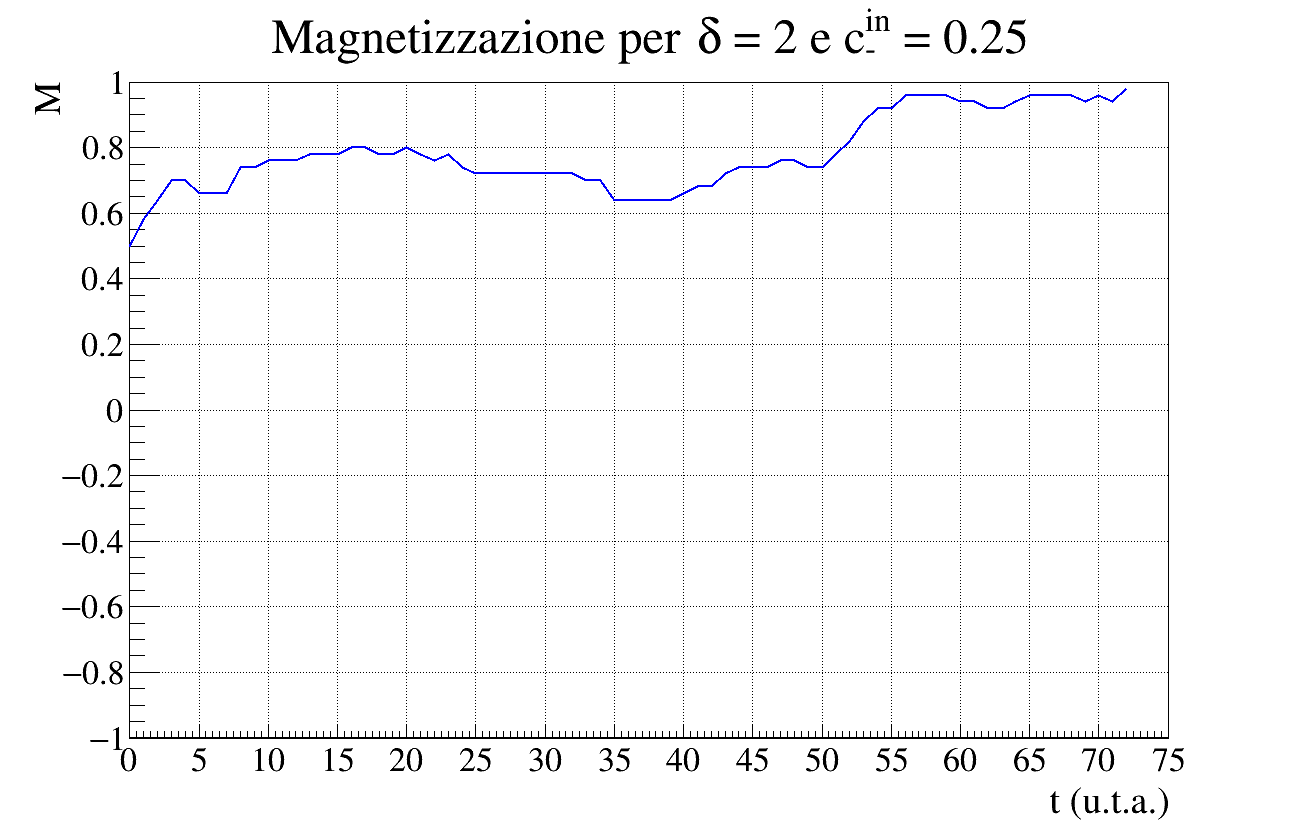
\includegraphics[width = 1.1\linewidth]{poland_sim_magnetization_graph.png}
\caption{\textit{bla bla bla}}
\label{Fig:9}
\end{figure}

\section{Implementazione}
\label{Sec:5}
Qui di seguito è riportato il codice python utilizzato per l'implementazione del modello. Per l'esecuzione si rammenta di scaricare l'\textit{interpreter} di \textit{python (v ${>=}$3.10)} compatibile con il proprio sistema operativo. Inoltre è necessario avere installato le librerie richieste, in caso contrario sono facilmente reperibili utilizzando dei \textit{package manager} come ad esempio \textit{pip}.

\section{Conclusioni}
\label{Sec:6}

\section{Bibliografia}
\label{Sec:7}

\end{document}
